\artigotrue
\chapter{THE SANTA MARIA DATASET. PART II -- COVARIATE DATA}
\chapternote{This chapter is based on the studies \textit{Identifying and correcting oblique striping in the 
Topodata digital elevation model}, presented at the XXXIV Brazilian Congress of Soil Science 
\cite{Samuel-RosaEtAl2013c}, and \textit{Evaluation of freely available ancillary data used for detailed soil 
mapping in Brazil}, presented at the EGU General Assembly 2014 \cite{Samuel-RosaEtAl2014}. Also collaborated 
in the preparation of this document: Pablo Miguel (UFPel), Jean Michel Moura Bueno (UFSM), Ricardo Simão Diniz 
Dalmolin (UFSM), Lúcia Helena Cunha dos Anjos (UFRRJ), Gustavo de Mattos Vasques (Embrapa Solos), and Gerard 
B. M. Heuvelink (ISRIC -- World Soil Information).}
\shorttitle{Covariate Data}
\label{chap:chap05}
%\SweaveUTF8



\def\ptkeys{Mapas areais de classes de solo. Modelos digitais de elevação. Mapas geológicos. Mapas de uso da 
terra. Imagens de satélite}
\begin{chapterabstract}{brazilian}{\ptkeys}
O \emph{conjunto de dados de Santa Maria} compreende uma lista de mais de $p = 100$ covariáveis espacialmente 
exaustivas produzidas nos 1980s, 1990s, and 2000s cobrindo a bacia do reservatório do Departamento Nacional de 
Obras de Saneamento-Companhia Riograndense de Saneamento (DNOS-CORSAN), localizada no estado sulista 
brasileiro do Rio Grande do Sul. Essas covariáveis foram derivadas de cinco fontes disponíveis gratuitamente 
em dois níveis de detalhe espacial: mapas areais de classes de solo (escala cartográfica de 1:\num{100000} e 
1:\num{25000}), modelos digitais de elevação (dados orbitais de radar com resolução espacial de \SI{90}{\m} e 
dados de curvas de nível com escala cartográfica de 1:\num{25000}), mapas geológicos (escala cartográfica de 
1:\num{50000} e 1:\num{25000}), mapas de uso da terra (escala cartográfica de 1:\num{25000} e 1:\num{2000}), e 
imagens de satélite (resolução espacial de 30 e \SI{5}{\m}). Esses dados de covariáveis são o resultado de 
projetos que visaram modelar várias características ambientais e foram realizados como parte de iniciativas 
locais (solo, geologia, uso da terra), regionais (terreno, uso da terra) e globais (terreno, uso da terra) de 
mapeamento. Os dados de covariáveis estão disponíveis gratuitamente em uma base de dados do GRASS GIS 
hospedada nos servidores do MEGAsync, enquanto o código-fonte utilizado na sua produção e processamento está 
disponível gratuitamente em um repositório hospedado no GitHub.
\end{chapterabstract}

\def\enkeys{Area-class soil maps. Digital elevation models. Geologic maps. Land use maps. Satellite images}
\begin{chapterabstract}{english}{\enkeys}
The \emph{Santa Maria dataset} comprises a list of more than $p = 100$ spatially exhaustive covariates 
produced in the 1980s, 1990s, and 2000s covering the catchment of the reservoir of the \textit{Departamento 
Nacional de Obras de Saneamento}-\textit{Companhia Riograndense de Saneamento} (DNOS-CORSAN), located in the 
southern Brazilian state of Rio Grande do Sul. These covariates were derived from five sources that are freely 
available in two levels of spatial detail: area-class soil maps (cartographic scale of 1:\num{100000} and 
1:\num{25000}), digital elevation models (airborne radar data with \SI{90}{\m} spatial resolution and 
contour line data at a \scale{25000}), geological maps (cartographic scale of 1:\num{50000} 
and 1:\num{25000}), land use maps (cartographic scale of 1:\num{25000} and 1:\num{2000}), and satellite images 
(30 and \SI{5}{\m} spatial resolution). These covariate data are the outcome of projects that aimed at 
modelling various environmental features and were carried out as part of local (soil, geology, land use), 
regional (terrain, land use), and global (terrain, land use) mapping initiatives. The covariate data is freely 
available in a GRASS GIS database hosted in MEGAsync servers, while the source code used in its production and 
processing is freely available in a repository hosted in GitHub.
\end{chapterabstract}

\formatchapter

\section{INTRODUCTION}
\label{sec:chap05-intro}

The \emph{Santa Maria dataset} is a data set comprising spatially exhaustive covariate data produced in the 
1980s, 1990s, and 2000s covering the catchment of the reservoir of the \textit{Departamento Nacional de Obras 
de Saneamento}-\textit{Companhia Riograndense de Saneamento} (DNOS-CORSAN), henceforth called \emph{DNOS 
catchment}, located in the southern border of the plateau of the Paraná Sedimentary Basin, in the city of 
Santa Maria, state of Rio Grande do Sul, Brazil. Most of the covariate data cover only part of the DNOS 
catchment, mainly the northern sector, which has an area of \SI{\pm2000}{\hectare}, corresponding to 
\SI{\pm60}{\percent} of the entire catchment. These covariate data are the outcome of projects that aimed at 
modelling various environmental features and were carried out as part of local (soil, geology, land use), 
regional (terrain, land use), and global (terrain, land use) mapping initiatives.

This chapter presents a thorough description of the covariate data contained in the Santa Maria dataset. 
These are area-class soil maps, digital elevation models, geological maps, land use maps, and satellite 
images. A thorough description of the procedures for their production, as well as the processing methods 
employed is given. The original sources of the covariate data are freely available at the producers databases 
or in public libraries.

The chapter is divided in seven sections. \autoref{sec:chap05-database} presents general information about 
the covariates, as well as the structure of the database where they have been stored and managed. Next, 
\autoref{sec:chap05-gcp} describes how ground data was collected to help processing and validating the 
existing covariate data. Area-class soil maps included in the Santa Maria dataset are described in 
\autoref{sec:chap05-soil-maps}, while \autoref{sec:chap05-dem} deals with the digital elevation models. 
Geologic maps and land use maps are described in \autoref{sec:chap05-geo-maps} and 
\autoref{sec:chap05-land-use}, respectively. \autoref{sec:chap05-sat-image} closes the chapter with a 
description of the satellite images included in the Santa Maria dataset.

\section{DATABASE STRUCTURE}
\label{sec:chap05-database}

Preparing the covariate data to enter the Santa Maria dataset required creating two databases. The first 
contains only vector (point) data, specifically point ground control data, as well as the code used in its 
processing. This database is freely available in the web-based \git{} repository \github{}. This is the same 
repository containing the soil data (\autoref{sec:chap04-database}). The repository has the following folder 
structured:

\begin{verbatim}
dnos-sm-rs-general
|- code/              # source code folder
|  - R/               # R source code folder
|    - general.R      # R source code file
|
|- data/              # data folder
|  - gcpData.csv      # ground control data file
|  - gcpMetadata.csv  # ground control metadata file
|- README.md          # description of the repository
\end{verbatim}

\def\sirgas{\href{http://spatialreference.org/ref/epsg/31982/}{\texttt{EPSG:31982}}}

Ground control data files are available as comma-separated values (CSV) files. The identification of all 
observation locations, their geographic coordinates, and elevation data are contained in the file 
\texttt{gcpData.csv}. File \texttt{gcpMetadata.csv} contain the metadata. The coordinate reference system 
(CRS) is \texttt{SIRGAS 2000 / UTM zone 22S}, coded \sirgas{} by the European Petroleum Survey Group 
(\href{http://www.epsg.org/}{EPSG}).

\def\megasync{\href{https://mega.nz/\#F!aY5CRQqY}{MEGAsync}}

% Footnote %%%%%
\def\footgrass{\footnote{Detailed information about the structure of a GRASS GIS database can be found in 
GRASS GIS \href{https://grass.osgeo.org/grass64/manuals/helptext.html}{help pages}.}}

The second database contains both vector (point, line and polygon) and raster (image) data. This database is 
freely available in \megasync{} servers, and is structured as a GRASS GIS database\footgrass{}. The database 
has the following folder structured:

\begin{verbatim}
dbGRASS               # GRASS GIS database
|- dnos-sm-rs         # Santa Maria dataset
|  - PERMANENT/          # general definitions folder
|  - predicitons/        # data folder
\end{verbatim}

\def\wgs{\href{http://spatialreference.org/ref/epsg/32722/}{\texttt{EPSG:32722}}}

All covariate data in the GRASS GIS database are harmonized to a reference grid of \SI{5}{\m} grid size. The 
CRS is \texttt{WGS1984 / UTM zone 22S}, coded \wgs{}.

\section{GROUND CONTROL POINTS}
\label{sec:chap05-gcp}

All covariates were validated prior to their use. Horizontal (positional) validation was performed using a set
of $n = 14$ validation points, here called ground control points (GCP), spread throughout and beyond the 
limits of the DNOS catchment (\autoref{fig:chap05-field-gcps}). The location of the GCPs was defined based on 
the existence of easily identifiable geographical markers across the covariates, including road intersection, 
fence corners, and property entrances.

\begin{figure}[!ht]
\centering
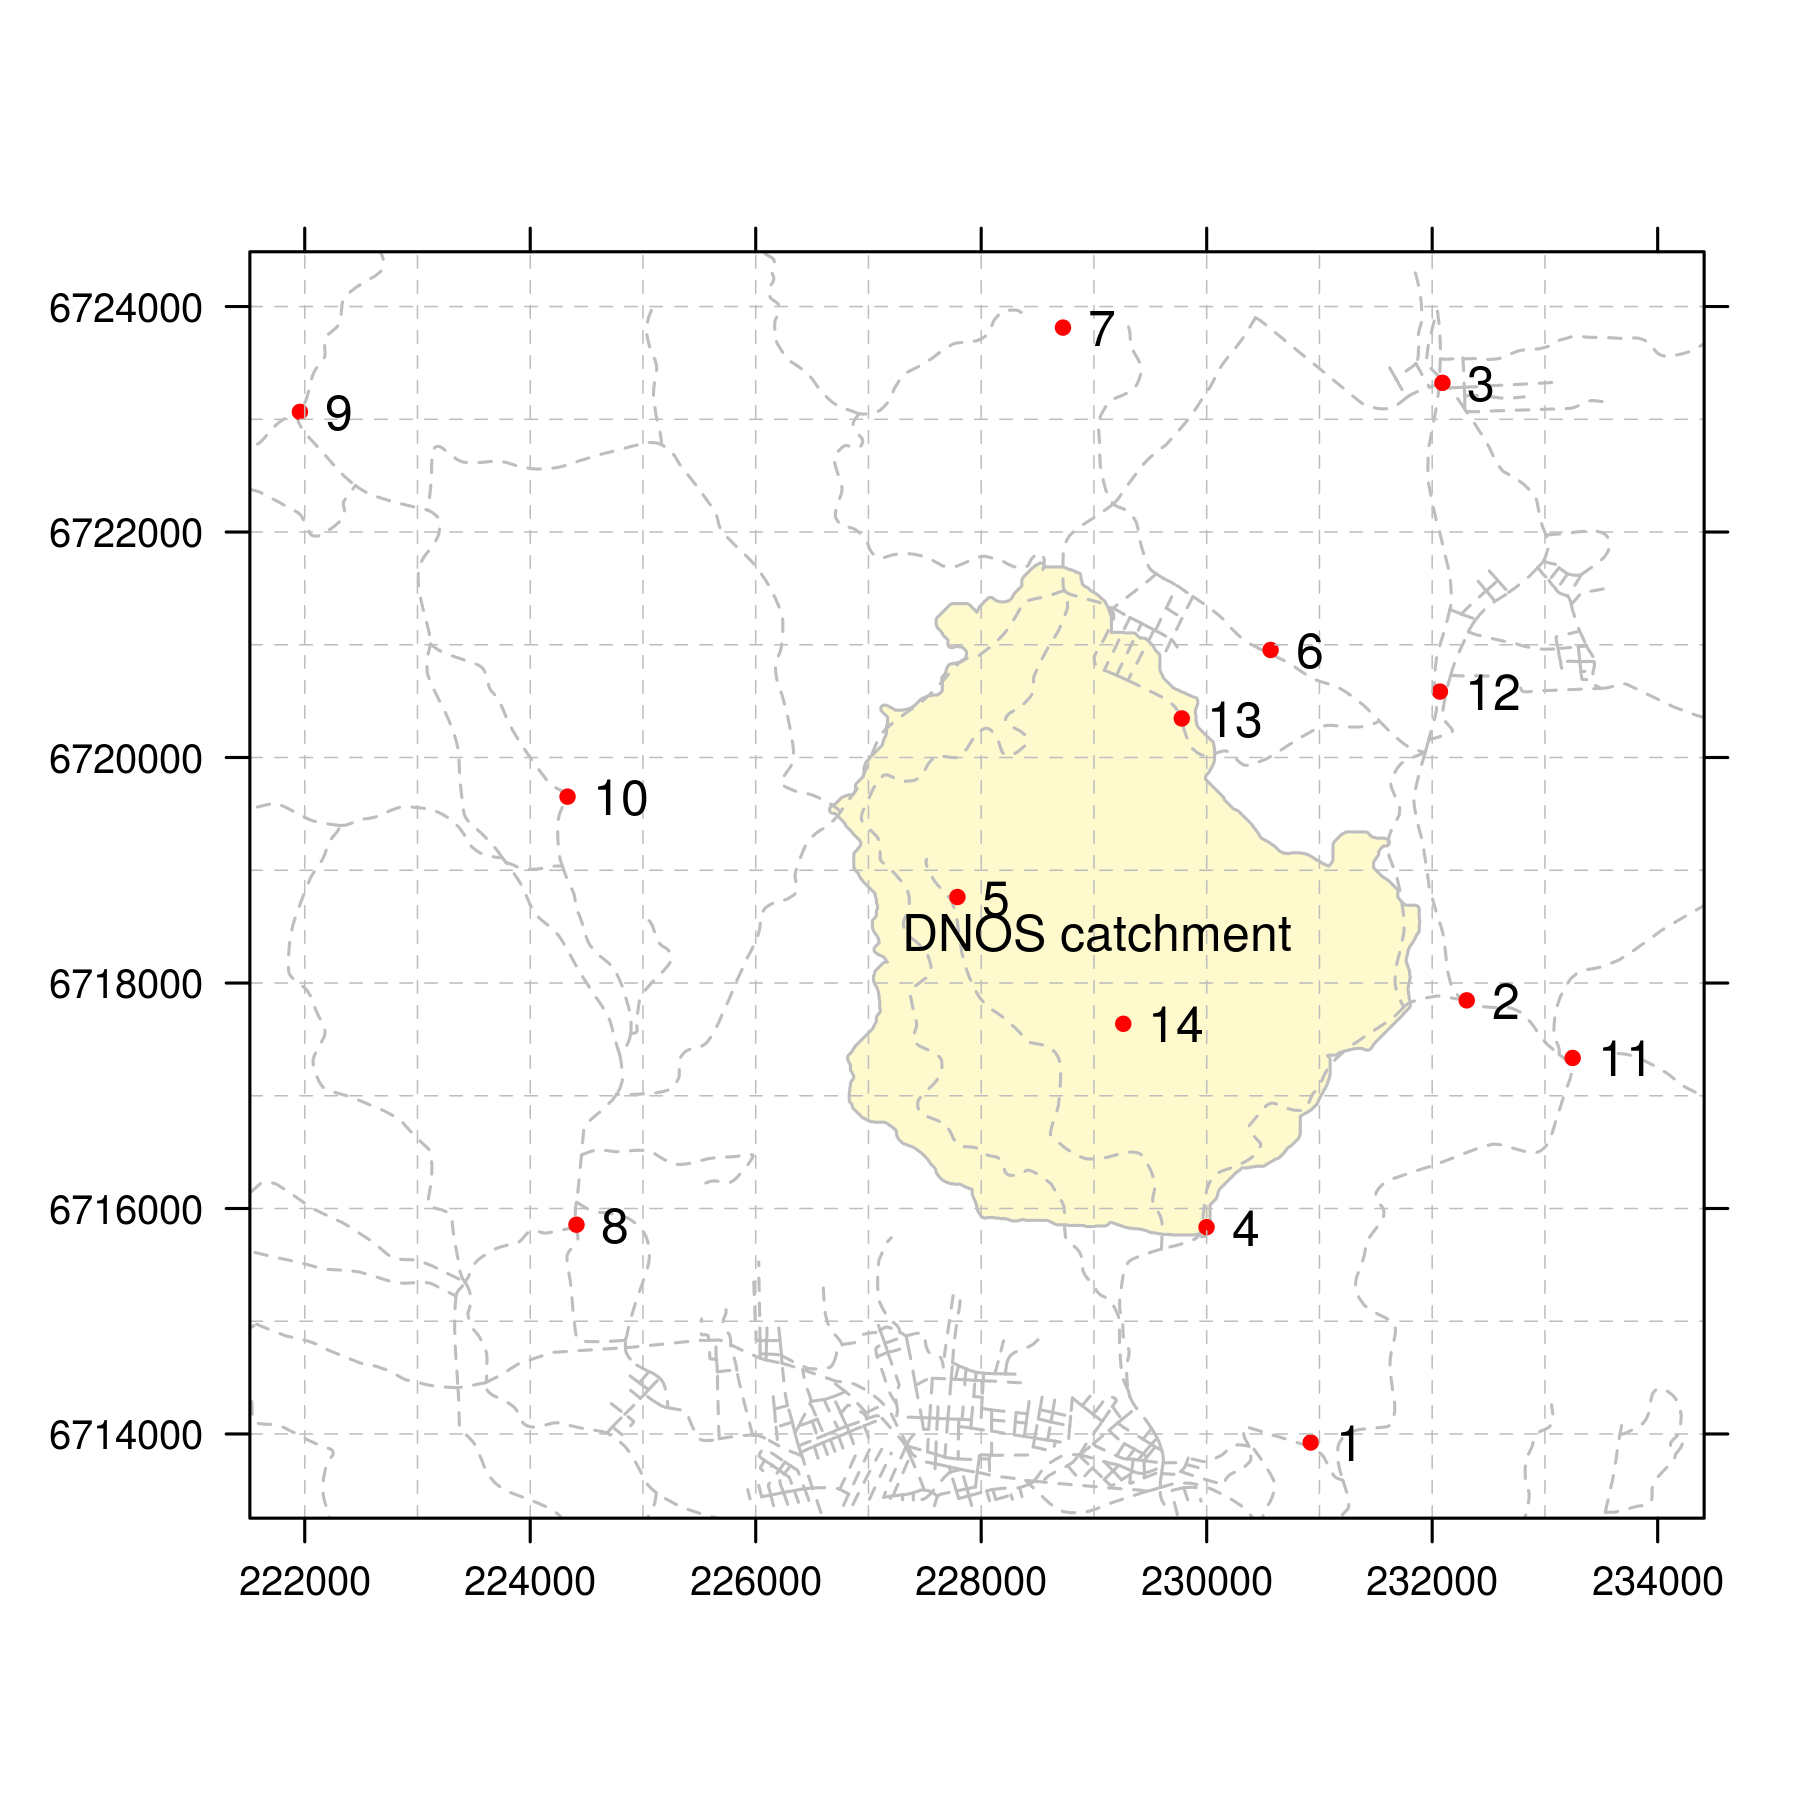
\includegraphics[width = 0.90\textwidth,trim=0 15mm 0 15mm, clip]{fig/chap05-field-gcps}
\caption[Ground control points used for the positional validation of the covariates.]{Spatial distribution of 
the ground control points ($n = 14$, red dots) used for the horizontal positional validation of covariates 
included in the Santa Maria dataset. The location of the ground control points is highly determined by the 
local road network (dashed grey line) surrounding the northern sector of the catchment of the reservoir of the 
\textit{Departamento Nacional de Obras de Saneamento}-\textit{Companhia Riograndense de Saneamento} (lemon 
chiffon-filled polygon).}
\label{fig:chap05-field-gcps}
\end{figure}

% TODO: Provide a more detailed description of how GCP data was collected and processed.

% TODO: Give a better description of how error measures were calculated.

Positional validation was performed comparing the x- and y-coordinates of GCPs (observed value) with the 
coordinates of the respective geographical markers visually identified on the covariates (predicted value). 
The differences in the observed and predicted x- and y-coordinates were used to calculate the mean error (ME, 
\si{\m}), mean absolute error (MAE, \si{\m}), and mean squared error (MSE, \si{\m\square}) to evaluate the  if 
there were differences in the accuracy and precision between coordinates. The error vector (or module, the 
euclidean distance between two points) and its azimuth (the orientation of the error vector) were computed as 
well for every point. The mean of the error vector and its azimuth give the size and orientation of the 
systematic error present in the covariates, while the square root of the mean squared error vector (RMSE) is a 
measure of the uncertainty about the true position of the covariate in the geographic space.

The field location of the GCPs is as follows:

\begin{description}
\item[GCP 01]
% Em Santa Maria, no lado direito da barragem de concreto do reservatório do DNOS-CORSAN, \SI{6}{\m} antes de 
% chegar a ponte sobre o vertedouro, a \SI{3}{\m} de distância do centro da estrada que desce da rodovia 
% federal BR158.
In Santa Maria, on the right side of the concrete dam of the DNOS-CORSAN reservoir, \SI{6}{\m} 
before reaching the bridge over the spillway, distant \SI{3}{\m} from the centre of the road that descends 
from the BR-158 federal highway.

\item[GCP 02]
% Em Itaara, na entrada da Estrada do Perau, Rua Gralha Azul, no centro do canteiro, entre o outdoor e a árvore 
% (\textit{Cedrella fissilis}), junto à rodovia federal BR158.
In Itaara, at the entrance of the Estrada do Perau, Rua Gralha Azul, in the centre of the roundabout, between 
the outdoor and the tree (\textit{Cedrella fissilis}), close to the BR-158 federal highway.

\item[GCP 03]
% Em Itaara, próximo ao equipamento estático de fiscalização eletrônica de velocidade, na rodovia federal 
% BR158, a \SI{520}{\m} do Museu de Ufologia, em frente à Fruteira da Esquina, do lado oposto da torre de 
% telefonia celular e da entrada para a mina de extração de brita DallaPasqua, localizada a \SI{4}{\km} do 
% local.
In Itaara, near the speed monitoring radar of the BR-158 federal highway, distant \SI{520}{\m} from the UFO 
Museum, opposite the Fruteira da Esquina, opposite to the cell phone tower and to the entrance of the gravel 
pit DallaPasqua, located \SI{4}{\km} away from the site.

\item[GCP 04]
% Em Santa Maria, na entrada da rua que dá acesso ao cemitério do Bairro Campestre do Menino Deus, no lado 
% direito da Estrada do Perau em direção à rodovia federal BR158, alinhado com a fachada das residências, a 
% \SI{2,2}{\m} de distância do muro frontal, a \SI{6,5}{\m} de distância do meio-fio da Estrada do Perau, a 
% \SI{50}{\m} de distãncia da ponte sobre o Rio Vacacaí-Mirim.
In Santa Maria, at the entrance of the street that leads to the cemetery of the Campestre do Menino Deus 
neighbourhood, on the right side of Perau Road going towards the BR-158 federal highway, aligned with the 
façade of the residences, \SI{2.2}{\m} away from the front wall, \SI{6.5}{\m} away from the curb of the Perau 
Road, \SI{50}{\m} away from the bridge over the Vacacaí-Mirim River.

\item[GCP 05]
% Em Santa Maria, na entrada do Rancho do Amaral, junto à porteira, no lado direito, fora da estrada, distante 
% \SI{1}{\m} de uma palmeira e \SI{1}{\m} do muro de pedras.
In Santa Maria, at the entrance of the Rancho do Amaral, next to the gate, on the right size, off the road, 
\SI{1}{\m} away of a palm tree and \SI{1}{\m} away from the stone wall.
 
\item[GCP 06]
% Em Itaara, na Avenida Etelvina, na beira da estrada, a \SI{2,5}{\m} de distância do centro da estrada,
% alinhado com a cerca que separa a floresta nativa do pomar de \textit{Citrus}~sp.~localizado do outro lado 
% da estrada.
In Itaara, Etelvina Avenue, on the roadside, \SI{2.5}{\m} away from the road centre, aligned with the fence 
that separates the native forest from the \textit{Citrus}~sp.~orchard located across the road.

\item[GCP 07]
% Em Itaara, Localidade de Estação Pinhal, no lado esquerdo do acesso à mina de extração de brita DallaPasqua, 
% sob a rede de transmissão de eletricidade.
In Itaara, Estação Pinhal Locality, on the left side of the beginning of the road that gives access to the 
DallaPasqua gravel pit, under the electricity transmission network.

\item[GCP 08]
% Em Santa Maria, Distrito de Santo Antão, na entrada da estrada que dá acesso à Central de Tratamento de 
% Resíduos da Caturrita, em frente à Escola Municipal de Ensino Fundamental Intendente Manoel Ribas.
In Santa Maria, Santo Antão District, at the beginning of the road that gives access to the Caturrita Waste 
Treatment Centre, opposite the Municipal Elementary School Intendente Manoel Ribas.
 
\item[GCP 09]
% Em São Martinho da Serra, Localidade de Água Negra, na bifurcação da estrada que vem de Santa Maria e que dá 
% acesso à Localidade de Campinas, junto à parada de ônibus, no canteiro no meio da bifurcação, \SI{40}{\m} 
% distante do Piquete Laçador Jorge R.~da Silva, em frente ao Mercado do Ronaldo.
In São Martinho da Serra, Água Negra Locality, at the bifurcation of the road coming from Santa Maria and 
giving access to the Campinas Locality, close to the bus stop, at the roundabout in the middle of bifurcation, 
\SI{40}{\m} away from the Piquete Laçador Jorge R.~da Silva, in front of Ronaldo's Market.

\item[GCP 10]
% Em Santa Maria, na estrada em direção à São Martinho da Serra, depois da capela Santo Antão, no lado externo 
% de uma curva, próximo a duas pequenas árvores, alinhado com a cerca que marca a divisa entre duas 
% propriedades ocupadas com campo nativo. Em frente à propriedade com duas residências, uma delas com dois 
% andares e quatro pequenos lagos nos fundos.
In Santa Maria, on the road towards São Martinho da Serra, after Santo Antão Chapel, on the outside of a 
curve, near two small trees, aligned with the fence that marks the boundary between two properties occupied 
with native grass. In front of the property with two houses, one with two floors and four small lakes in the 
backyard.
 
\item[GCP 11]
% Em Itaara, entrada para a Localidade Rincão dos Minello, no início da estrada que dá acesso à Brita Pinhal, 
% ao lado da rodovia federal BR158, \SI{5}{\m} de distância à frente do corte no terreno expondo a rocha de 
% arenito da Formação Botucatu, \SI{15}{\m} distante do poste da linha de transmissão de eletricidade da 
% companhia AES.
In Itaara, at the entrance to the Rincão dos Minello Locality, at the beginning of the road that gives access 
to Brita Pinhal, next to the BR-158 federal highway, \SI{5}{\m} away and in front of the road cut exposing the 
sandstone rocks of the Botucatu Formation, \SI{15}{\m} away from the post of the electricity transmission line 
of the AES company.

\item[GCP 12]
% Em Itaara, na rodovia federal BR158, em frente ao lago da SOCEPE, na entrada da cidade, próximo ao Bar e 
% Armazém Ricardo, deslocado em \SI{1}{\m} para dentro do passeio em relação ao alinhamento dos postes da rede 
% elétrica.
In Itaara, at the federal highway BR-158, in front of the SOCEPE's Lake, in the city entrance, near the 
Ricardo's Bar and Warehouse, shifted \SI{1}{\m} into the side walk in relation to the alignment of the posts 
of the electrical network.

\item[GCP 13]
% Em Itaara, na Vila Etelvina, com uma vinha à montante, alinhado com a cerca que divide duas propriedades 
% localizadas no lado oposto da estrada, uma à esquerda coberta com floresta nativa/exótica e outra à direita 
% ocupada com lavoura de culturas anuais.
In Itaara, at Vila Etelvina, with a vineyard upstream, aligned with the fence that divides two properties 
located on the opposite side of the road, the one on the left covered with native/exotic woods and the other 
on the right occupied with field of annual crops.
 
\item[GCP 14]
% Em Itaara, na estrada que sobe para a propriedade do Sr. Antoninho Luccas, logo após o término da subida 
% íngreme com calçamento apenas nos trilhos, no final da floresta e início do campo nativo, alinhado (a 
% \SI{20}{\cm}) com a cerca dos dois lados da estrada. Locado \SI{1}{\m} distante do moirão da cerca do lado 
% esquerdo subindo, no interior da estrada.
In Itaara, in the road that goes towards the property of Mr.~Antoninho Luccas, soon after the steep climb, 
where there is only pavement on the tracks, at the end of the forest and beginning of native grass, aligned 
with the fence on both sides of road, \SI{1}{\m} away from the left corner fence post.
\end{description}

Attribute validation of soil, geologic, and land use maps, and digital elevation models was done using a set 
of $n = 60$ validation points located along $m = 12$ linear transects (\autoref{sec:chap04-subset-ii}). The 
procedures for obtaining soil, geologic, land use, and elevation data at these validation points is described 
in \autoref{sec:chap04-field-description}. Such a validation exercise was carried out because these maps 
originally had no accompanying validation information.

% TODO: figure with GCPs used to orthorectify satellite images.

% Show the bounding box of the image and the boundary of the study area.
% \begin{figure}
%  \centering
%  \includegraphics[width=\textwidth]{fig/ortho-gcps}
%  \caption{Ground control points used to orthorectify the image produced by Landsat-5 Thematic Mapper.}
%  \label{fig:chap05-ortho-gcps}
% \end{figure}

\section{AREA-CLASS SOIL MAPS}
\label{sec:chap05-soil-maps}

Two area-class soil maps are included in the Santa Maria dataset. The first of them (\soilOld{}, 
\autoref{fig:chap05-soil-old}) was published at a \scale{100000} \cite{AzolinEtAl1988}. Existing area-class 
soil maps and technical reports \cite{Brasil1973, Azolin1977, MacielEtAl1987a, MacielEtAl1987, AbraoEtAl1988}, 
and sparse field observations were used to elaborate the preliminary legend of the soil map. Aerial 
photographs (\scale{60000}) were used to produce the first draft of the soil map. Field checks of soil 
polygons (i.e. mapping units) was done along the road network (i.e. by convenience sampling). These 
observations were used to estimate the composition (occurrence and spatial distribution of soil taxa) of soil 
mapping units. They were also used to review the first draft of the soil map. The final version of \soilOld{} 
was prepared using topographic maps originally published at a \scale{50000} and resampled to a \scale{100000}. 
Soil classification followed the criteria adopted by the Brazilian soil science community at that time 
\cite{Brasil1973, CamargoEtAl1982, Carvalho1982, LemosEtAl1982, OlmosEtAl1982}. Identification of soil taxa 
was performed based on morphological features, analytical data compiled from existing technical reports, and 
analysis of soil samples collected from soil profiles observed along the road network. Description of each 
soil mapping unit includes the estimated area (\si{\hectare}) and the approximate taxonomic composition 
(\si{\percent}).

\begin{figure}[!ht]
\centering
\begin{minipage}[b]{0.45\textwidth}
\subcaption{}
\label{fig:chap05-soil-old}
\centering
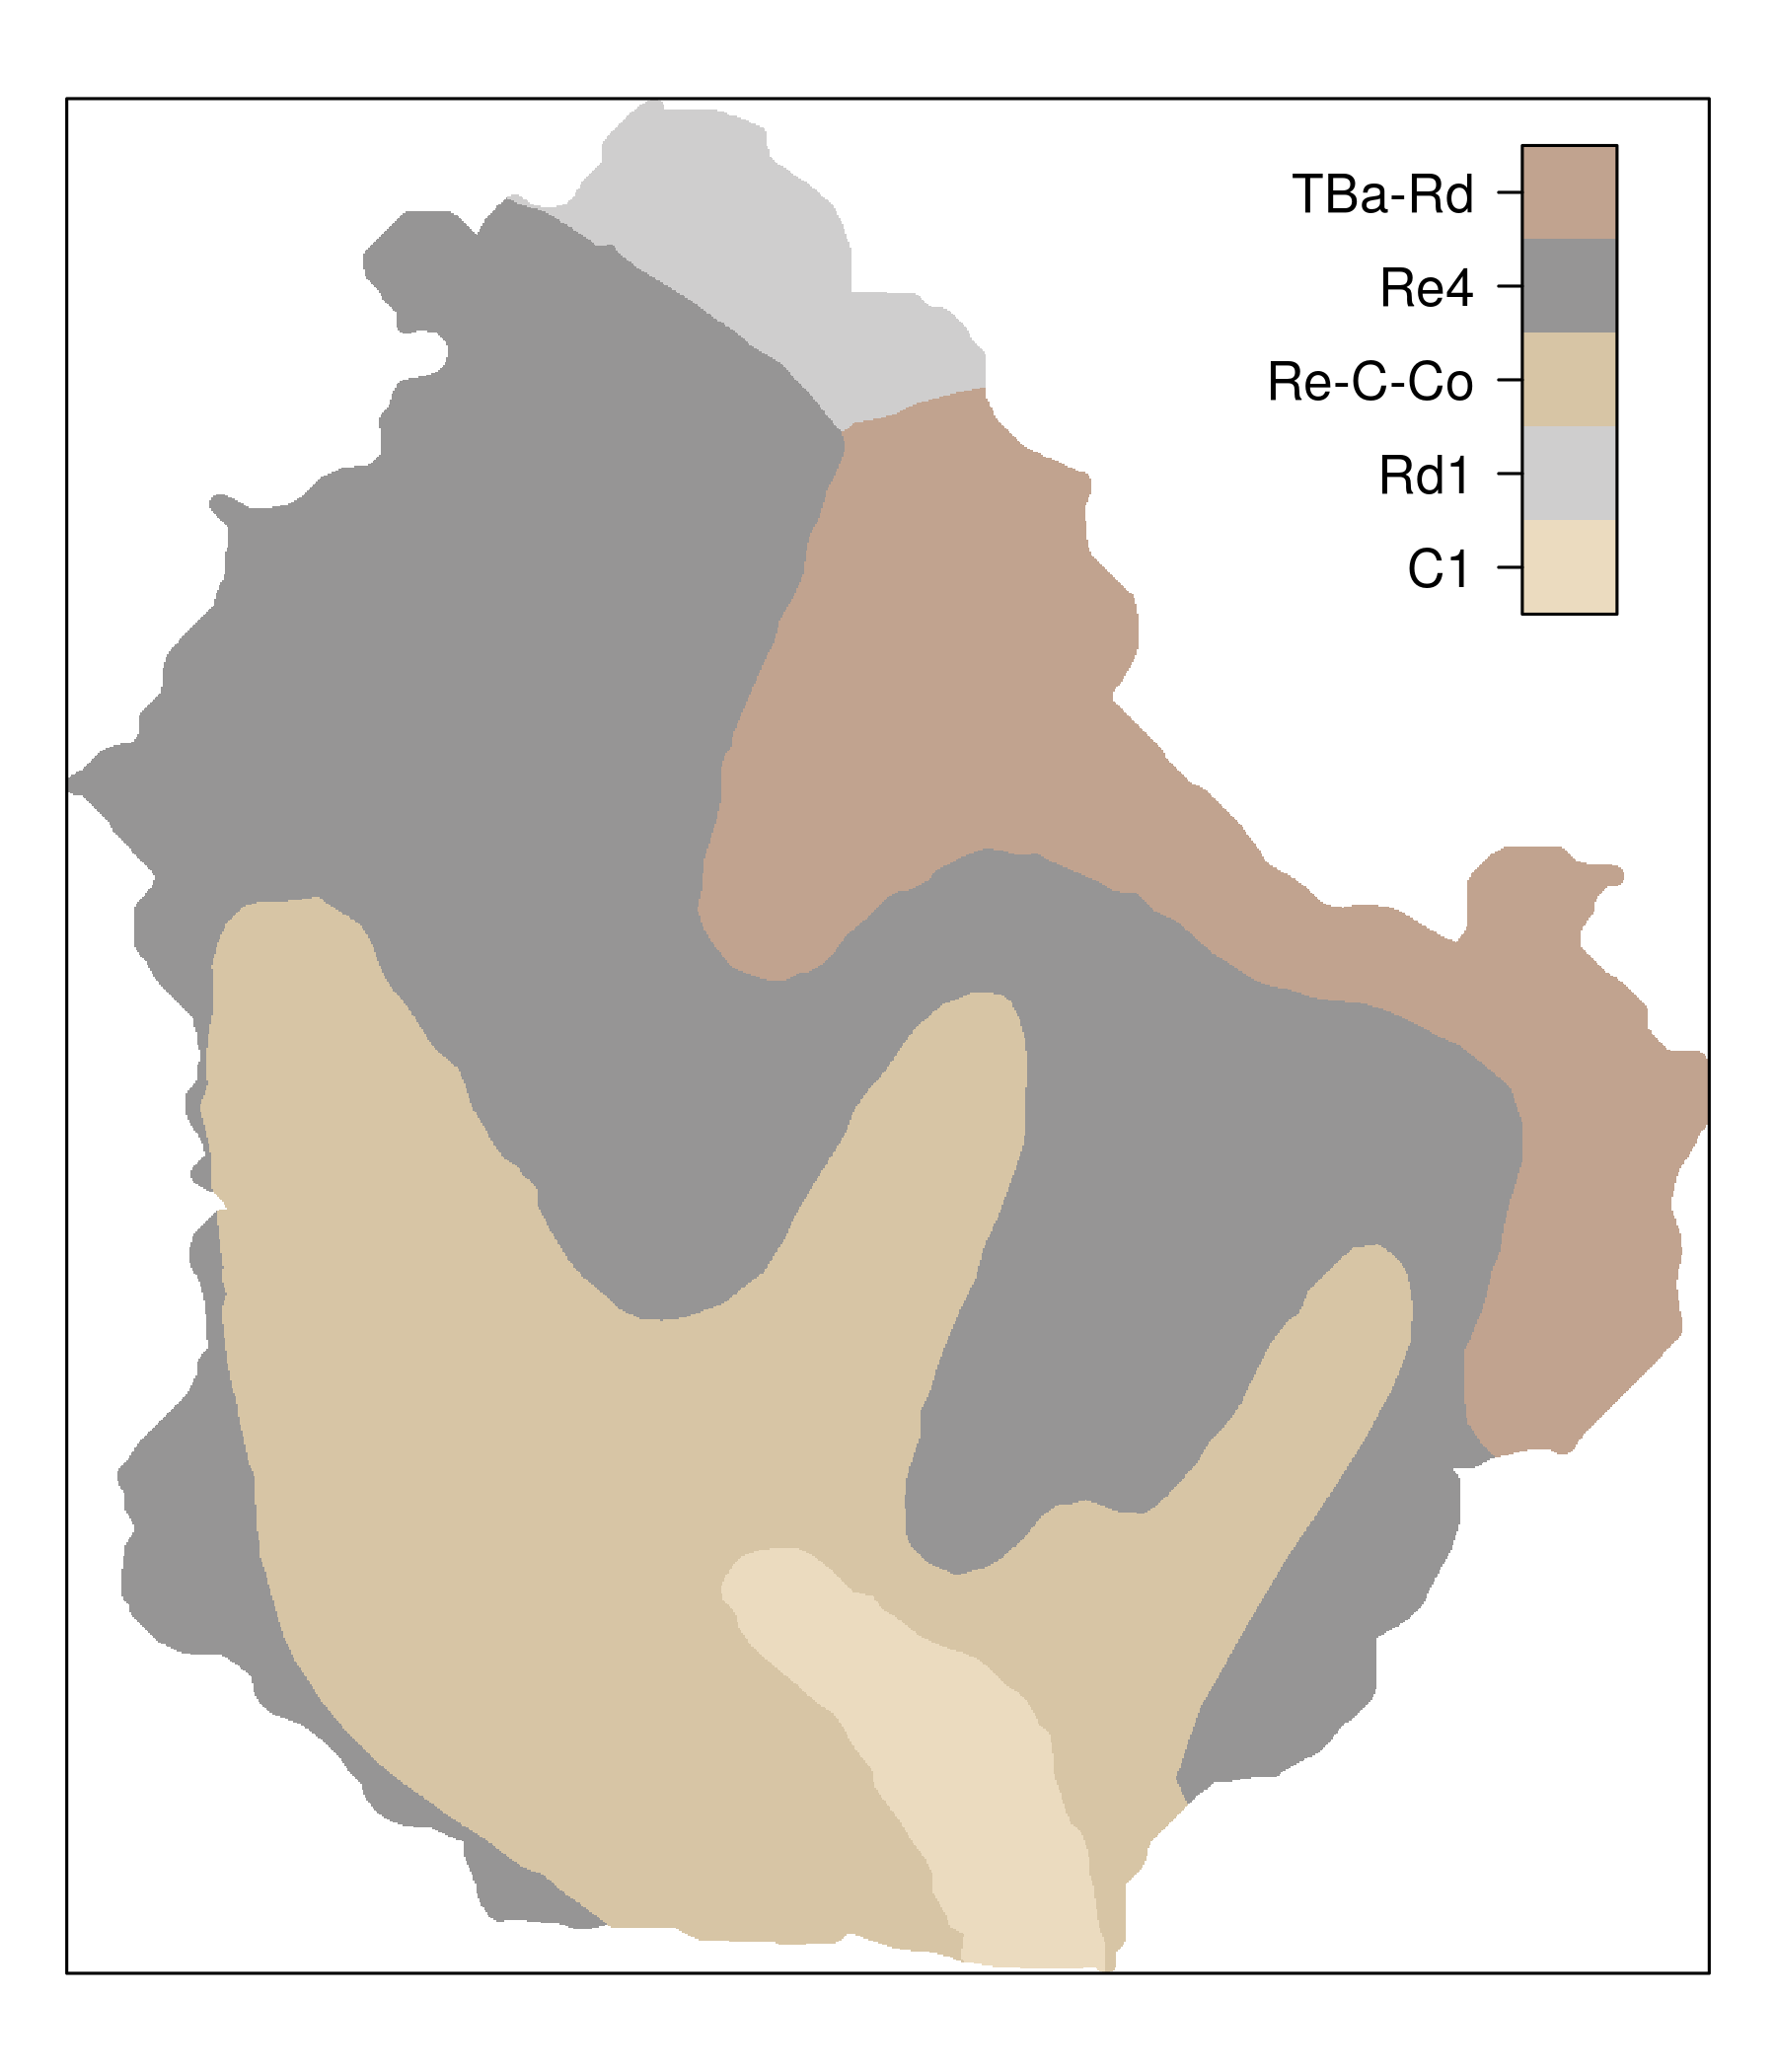
\includegraphics[width = \textwidth]{fig/chap05-soil-old}
\end{minipage}
\begin{minipage}[b]{0.45\textwidth}
\subcaption{}
\label{fig:chap05-soil-new}
\centering
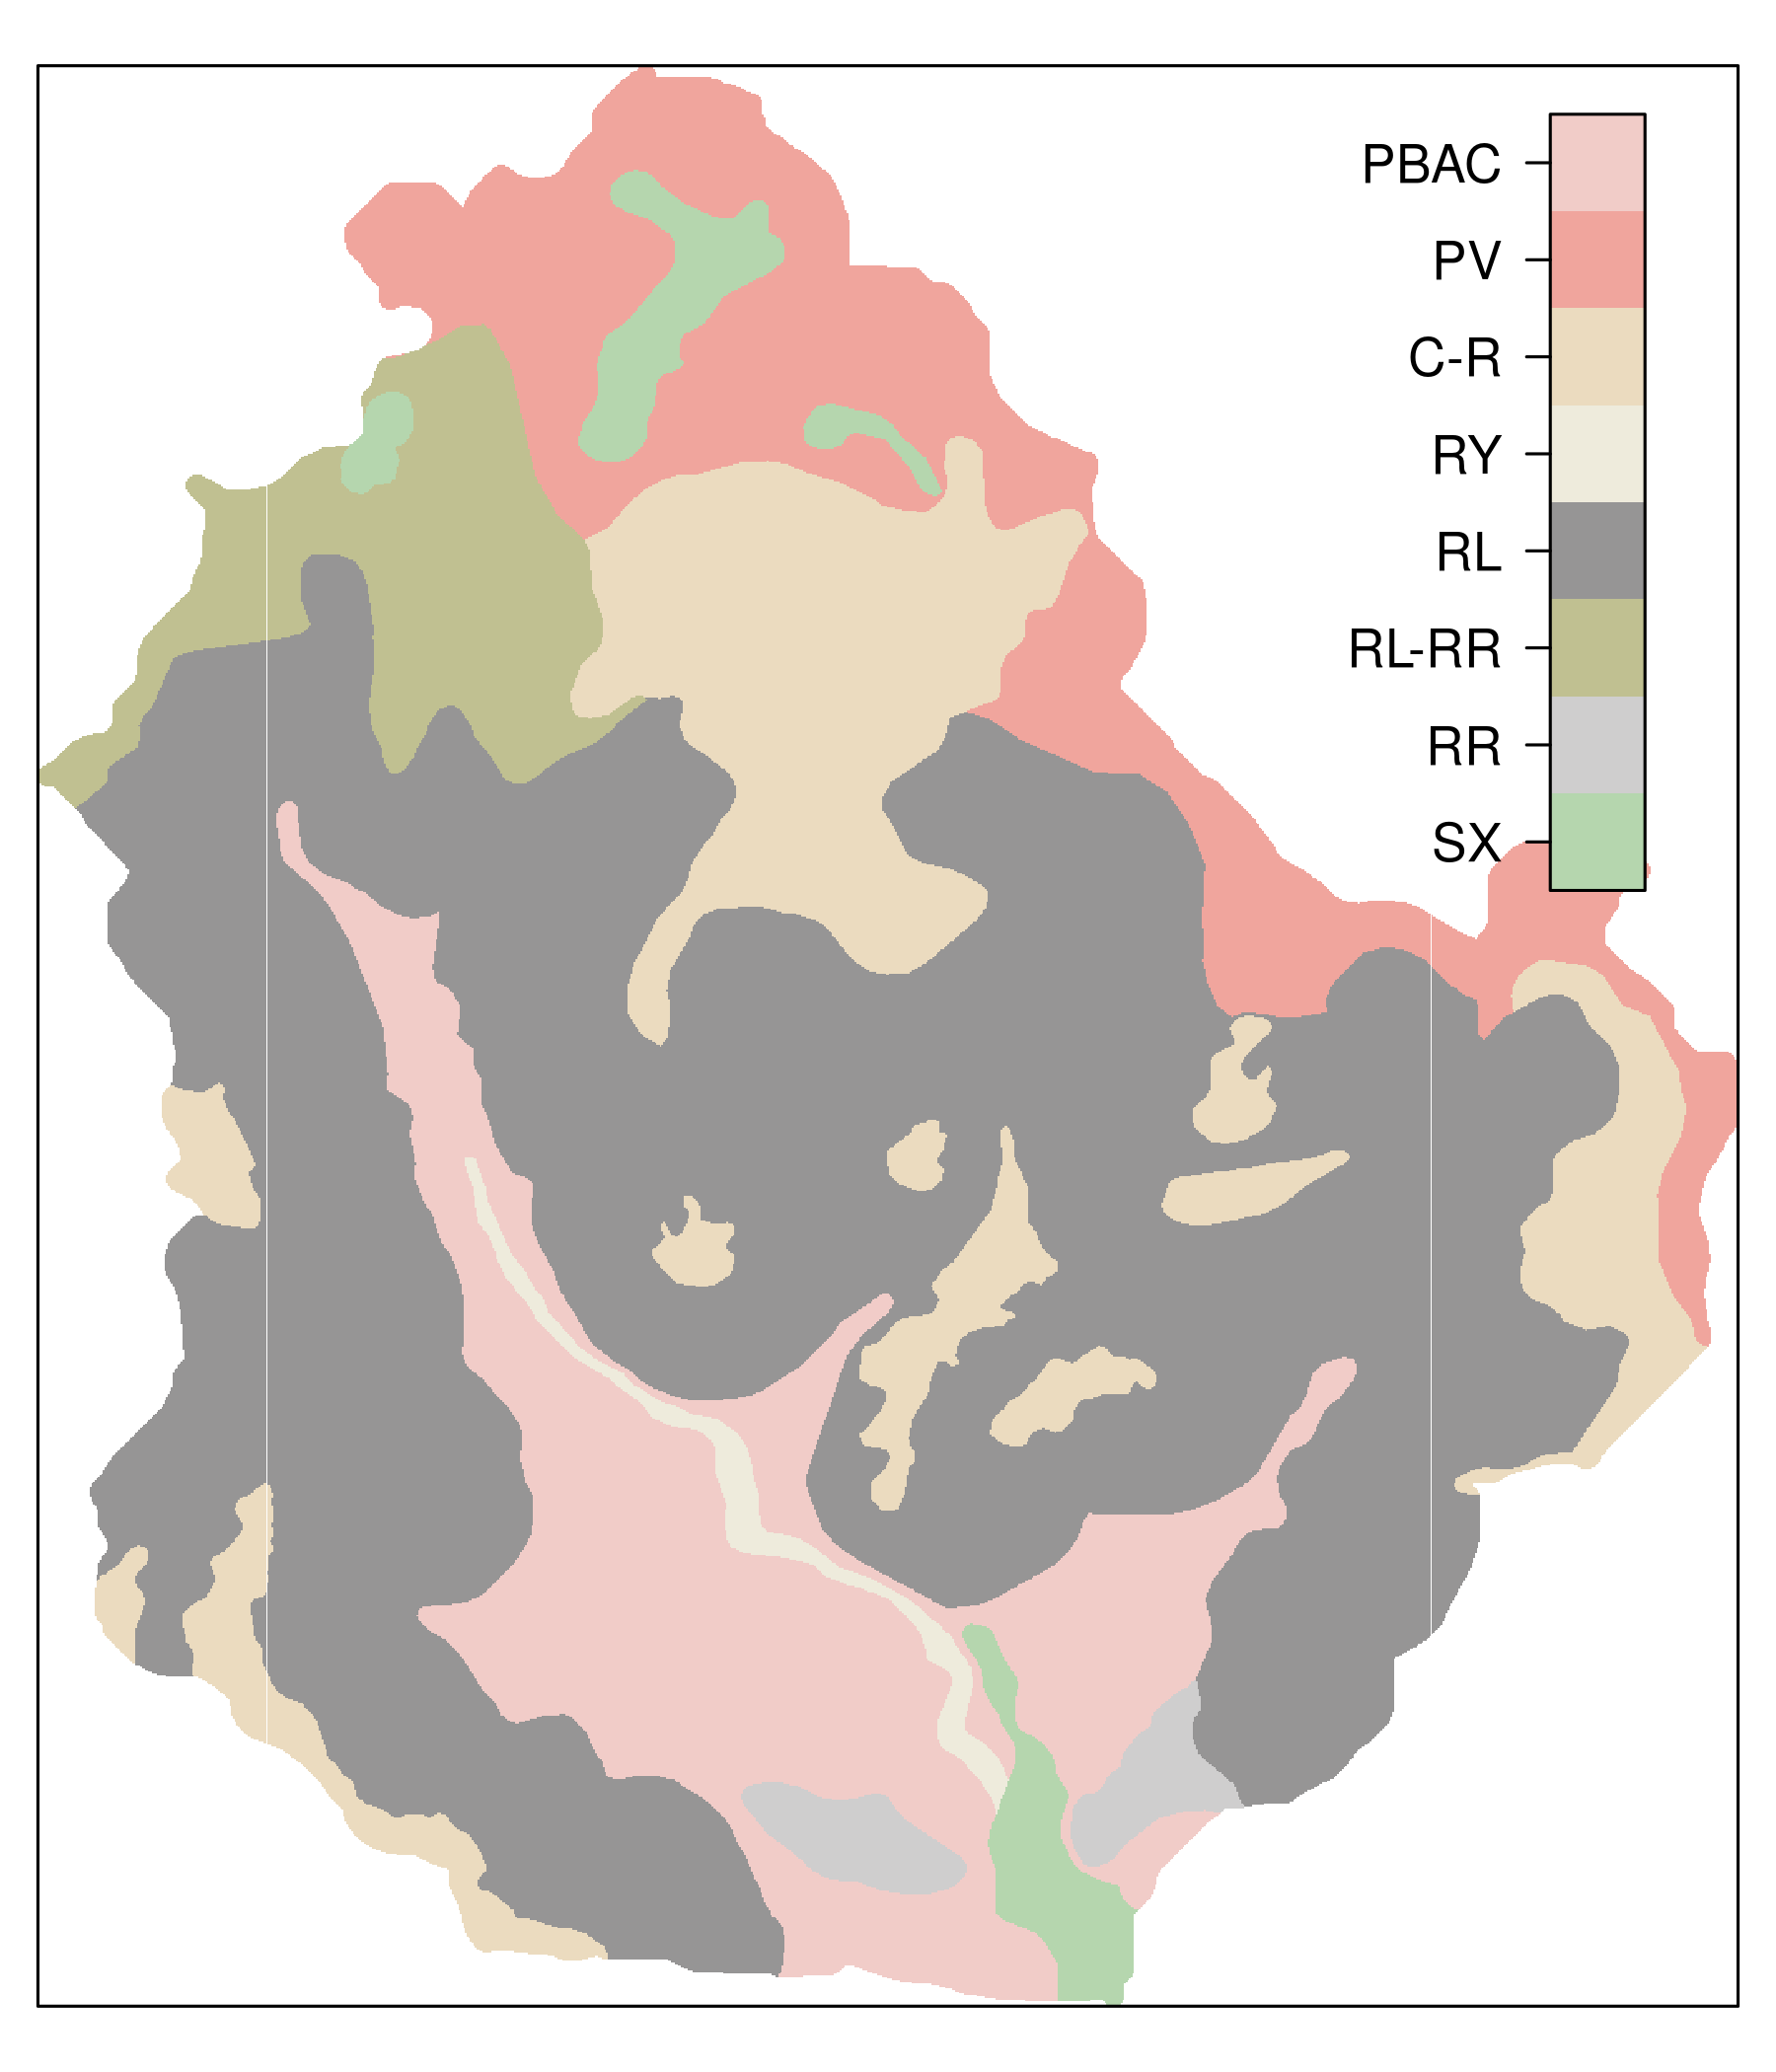
\includegraphics[width = \textwidth]{fig/chap05-soil-new}
\end{minipage} 
\caption[Area-class soil maps included in the Santa Maria dataset.]{Area-class soil maps (a) \soilOld{} and 
(b) \soilNew{} used to derive indicator covariates included in the Santa Maria dataset. Legend abbreviations 
and derived indicator variables are described in the text.}
\label{fig:chap05-soil-maps}
\end{figure}

% Footnote %%%%%
\def\footquick{\footnote{Detailed information about the Digital Globe\rr{} QuickBird satellite can be found 
in \href{https://en.wikipedia.org/wiki/QuickBird}{Wikipedia}.}}

The second area-class soil map (\soilNew, \autoref{fig:chap05-soil-new}) included in the Santa Maria dataset 
\cite{Miguel2010} was prepared at a \scale{25000}. Satellite images of the year of 2009, with 
\SI{2.4}{\m}-spatial resolution, produced by the Digital Globe\rr{} QuickBird satellite\footquick{}, freely 
available for visualization in Google Earth\rr{}, were used to produce the first draft of the soil map. 
Existing area-class soil maps and technical reports \cite{Pedron2005, Poelking2007, Sturmer2008} were used to 
help defining the preliminary soil map legend. Field observations (soil pits and boreholes) were made in 
more than \num{350} locations using a purposive sampling approach (see \autoref{chap:chap04} and 
\autoref{chap:chap07}). These observations helped to identify six modal (representative) soil profiles. Soil 
sampling and description of modal soil profiles, and laboratory analyses of soil samples, followed the 
standard protocols adopted in Brazil \cite{ClaessenEtAl1997, SantosEtAl2005}. Soil classification was 
performed following the criteria of the Brazilian System of Soil Classification (SiBCS) \cite{SantosEtAl2006}. 
The final version of the map was prepared using the same satellite images freely available for visualization 
in Google Earth\rr{} and manually-digitalized topographic sheets published at a \scale{25000} \cite{DSG1992a, 
DSG1992}. Description of soil mapping units includes only the most common soil taxon, followed by 
morphological and laboratory data of modal soil profiles.

The area-class soil maps went through different preprocessing routines. The original \soilOld{} is available 
only in analogical format, what required its digitalization. Georeferencing was carried out using the GDAL 
Georeferencer plug-in in QGIS \cite{GDAL2013, QGIS2013}. Intersections between all meridians and parallels 
($n = 9$) were used as control points to adjust a second order polynomial model. Resampling was performed 
using the cubic resampling method. Soil polygons and their attributes were also manually digitalized in QGIS. 
Because of the coarseness of the cartographic map scale (\scale{100000}), most geographical markers used to 
locate validation GCPs could not be identified and positional validation was performed using only $n = 4$ 
GCPs. Estimated error statistics suggest that there are large positional errors in all directions, with an 
RMSE of \SI{114}{\m} and a mean azimuth of \SI{128}{\degree} (\autoref{tab:chap05-soil-geo-val}).

\ctable[
  caption  = {Error statistics of the horizontal positional validation of \soilOld{} using $n = 4$ ground
  control points.},
  cap      = {Error statistics of the horizontal positional validation of \soilOld.},
  label    = tab:chap05-soil-geo-val,
  notespar,
  pos      = !ht,
  maxwidth = \textwidth,
  % doinside = \scriptsize\setstretch{1.1},
  doinside = \small
  ]{lrrrr}{
  }{                                                                          \FL
  Statistics                   & x-coord & y-coord & Error vector & Azimuth   \ML
  Mean, \si{\m}                & 30      & -36     & 105          & \ang{128} \NN
  Absolute mean, \si{\m}       & 58      & 64      & -            & -         \NN 
  Squared mean, \si{\m\square} & 7241    & 5712    & 12953        & -         \LL
  }

% \begin{figure}[!ht]
%   \centering
%   \includegraphics[width=0.45\textwidth]{azim-soil100}
%   \includegraphics[width=0.45\textwidth]{azim-soil25}
%   \caption{Histogram of the azimuth distribution of the validation of area-class soil maps \soilOld{} 
% and \soilNew{} in the attribute space. Azimuth values were estimated using four and XX
% ground control points located in easily identifiable geographical markers, respectively. 
% The graph was produced using R-package \textit{VecStatGraphs2D}.}
%   \label{fig:soil-azim}
% \end{figure}

The original \soilNew{} is available in digital format in the personal database of the author 
\cite{Miguel2010}. A topology check performed using the Topology Checker plug-in in QGIS identified that 
there were many gaps and overlaps between polygons. This required a topological edition prior to the use of 
\soilNew. There also was a mismatch between the boundary of \soilNew{} and the actual boundary of the study 
area as estimated using \demNew{} (\autoref{sec:chap05-dem}). This occurred because the database used to 
produce \soilNew{} included \SI{2.4}{\m}-spatial resolution Google Earth\rr{} imagery and topographic maps, 
which are data sources that differ considerably in their positional accuracy (\autoref{sec:chap05-dem} and 
\autoref{sec:chap05-land-use}). To avoid data losses, all boundary gaps were manually filled using the closest 
mapping unit. Boundaries of soil polygons were defined based on land use (\landNew{}, 
\autoref{sec:chap05-land-use}) and topographic data (contour lines, \autoref{sec:chap05-dem}) as it was done 
for the original map \cite{Miguel2010}. New delineations were checked and approved without modifications by 
the author of the original map. Because \soilNew{} includes very few geographical markers, its positional 
validation was not possible with the available GCPs. However, the RMSE is expected to vary between 
8 and \SI{114}{\m} across the DNOS catchment as a result of the different errors present in the data sources 
used in its production.

Both \soilOld{} and \soilNew{} were cropped to the bounding box of the DNOS catchment, and resampled to match 
the reference grid using the nearest neighbour resampling method to maintain data integrity. Each category was 
named with the code of the respective mapping unit in the original map. Prior to validation in the attribute 
space, class codes of \soilOld{} were changed to match soil taxa codes of the current Brazilian System of Soil 
Classification using a standard correlation table \cite{SantosEtAl2006}. The overall purities of both soil maps 
are not considerably different. A reason for this could be that validation was performed considering only the 
second level of the SiBCS -- it is likely that \soilNew{} would outperform \soilOld{} if validation data 
included soil taxa up to the fourth level of the SiBCS. The low overall purity of \soilOld{} and 
\soilNew{} (\num{31.67} and \SI{30.00}{\percent}, respectively) is likely due to several sources of error. 
First, the small number of modal soil profiles used to produce both maps that might have resulted in an 
optimistic view of the homogeneity of each mapping unit. Second, soil classes of \soilOld{} were translated to 
the more recent SiBCS using only a standard correlation table \cite{SantosEtAl2006} and expert knowledge 
because the survey report does not include analytical soil data. Last, soil classes at the $n = 60$ validation 
sites were inferred in the field using only morphological soil properties and the general concepts of the 
SiBCS.

Five ($p = 5$) covariates were derived from \soilOld{} as described below (including the soil classes 
according to the original and updated classification \cite{AzolinEtAl1988, SantosEtAl2013a}, and the 
international classification \cite{IUSSWorkingGroupWRB2007}):

\begin{description}
\item[\texttt{SOIL\_100b}] Shallow soil (\textit{Re4}) with low to high base saturation covering mountainous 
terrain (Solo Litólico Eutrófico/Distrófico relevo montanhoso; Neossolo Litólico Distrófico/Eutrófico;
Distric/Eutric Leptosol).
  
\item[\texttt{SOIL\_100c}] Association (\textit{Re-C-Co}) of shallow soil with high base saturation located in
steep terrain (Solo Litólico Eutrófico relevo forte ondulado; Neossolo Litólico Eutrófico; Eutric
Leptosol), low weathered soil (Cambissolo Eutrófico; Cambissolo Háplico Eutrófico; Eutric Cambisol), and
colluvial deposits.
  
\item[\texttt{SOIL\_100d}] Association (\textit{TBa-Rd}) of deep, well-structured, low base saturation soil 
(Terra Bruna Estruturada álica; Nitossolo; Nitisol), and shallow soil (Solo Litólico; Neossolo Litólico; 
Leptosol).
  
\item[\texttt{SOIL\_100e}] Shallow soil (\textit{Rd1} and \textit{Re4}) with low to high base
saturation (Solo Litólico Distrófico/Eutrófico; Neossolo Litólico Distrófico/Eutrófico; Distric/Eutric
Leptosol) located in undulating to mountainous terrain.
  
\item[\texttt{SOIL\_100f}] This covariate includes the best soil mapping units for row crop agriculture among 
those identified in the soil survey, that is \textit{TBa-Rd}, described above, and \textit{C1}, which is 
composed of low weathered soil developed in lower landscape positions, close to drainage channels (Cambissolo
Eutrófico; Cambissolo Háplico Eutrófico; Eutric Cambisol).
\end{description}

Covariates derived from \soilNew{} are presented below. Mapping unit \textit{RY}, composed mainly of soil 
developed from fluvial deposits (Neossolo Flúvico; Fluvisol) does not appear due to the small area that it 
occupies.

\begin{description}
\item[\texttt{SOIL\_25a}] Moderately deep soil (\textit{PBAC}) derived from sedimentary rocks, with abrupt 
textural change and low base saturation (Argissolo Bruno-Acinzentado; Alisol).

\item[\texttt{SOIL\_25b}] Deep soil (\textit{PV}) derived from igneous rocks, with moderate textural 
gradient, and low base saturation (Argissolo Vermelho; Acrisol).

\item[\texttt{SOIL\_25c}] Low weathered soil (Cambissolo Háplico; Cambisol) and shallow soil with low to high 
base saturation (Neossolo Litólico/Regolítico Eutrófico/Distrófico; Eutric/Distric Leptosol/Regosol) 
(\textit{C-R}).

\item[\texttt{SOIL\_25d}] Shallow soil (\textit{RL}) with low to high base saturation (Neossolo Litólico 
Eutrófico/Distrófico; Eutric/Distric Leptosol).

\item[\texttt{SOIL\_25h}] This covariate includes the mapping units with the best soils for row crop 
agriculture among those identified in the soil survey (\textit{PBAC}, \textit{PV}, and \textit{SX}). 
\textit{PBAC} and \textit{PV} are as described above. \textit{SX} is composed of moderately deep soil derived 
from sedimentary rocks, with abrupt textural change, low base saturation, and which are saturated with water 
for long periods of the year (Planossolo Háplico; Planosol).

\item[\texttt{SOIL\_25i}] This covariate includes all three mapping units (\textit{RL}, \textit{RL-RR}, and 
\textit{RR}) composed mainly of shallow soils (Neossolo Litólico and Neossolo Regolítico; Leptosol and 
Regosol).

\item[\texttt{SOIL\_25j}] This covariate includes all four mapping units (\textit{PV}, \textit{RL}, 
\textit{RL-RR}, and \textit{C-R}) composed mainly of soil derived from igneous rocks.
\end{description}

\section{DIGITAL ELEVATION MODELS}
\label{sec:chap05-dem}

Two digital elevation models (DEMs) are included in the Santa Maria dataset as sources of terrain covariates. 
The first DEM (\demNew, \autoref{fig:chap05-dem-old}) is the result of the interpolation of the contour lines 
of the most recent topographic sheets produced by the Brazilian Army (\scale{25000}) that cover the DNOS 
catchment \cite{DSG1980, DSG1992, DSG1992a}. Topographic sheets were digitalized and georeferenced using the 
GDAL Georeferencer plugin in QGIS. Intersections between all meridians and parallels (about $n = 160$ per 
topographic sheet) were used as control points to adjust a third order polynomial model. Resampling was 
performed using the cubic resampling method. All contour lines, peaks, lakes and rivers, and their respective 
attributes within a distance of \SI{1000}{\m} from the boundary of the DNOS catchment were manually digitized 
and stored in vector format. After digitalization, the original coordinate reference system (EPSG:31982 -- 
SIRGAS2000 / UTM zone 22S) of all vector files was transformed to WGS1984 / UTM zone 22S (EPSG:32722) using 
the \Rpackage{rgdal} \cite{BivandEtAl2013a}.

The horizontal positional validation of topographic maps was performed using the $n = 14$ GCPs. According to 
Brazilian legislation, high-quality map standards require that at least \SI{90}{\percent} of the GCPs have 
horizontal positional errors smaller than \SI{13}{\metre}, and an overall horizontal error (i.e. RMSE) smaller 
than \SI{8}{\metre} at the \scale{25000} \cite{Brasil1984}. Estimated validation statistics show that the 
overall observed horizontal error ($\text{RMSE} = \SI{65}{\m}$) is larger than those established by current 
regulations (\autoref{tab:chap05-topomap-geo-val}). The mean error vector is larger than \SI{60}{\metre} with 
an azimuth of \SI{63}{\degree}. Both x- and y-coordinates are positively biased, but the largest error occurs 
in the x-coordinate (\SI{50}{\metre}). Similar ME and MAE values suggests that there is a strong systematic 
positional error. An affine transformation was employed using the \Rpackage{vec2dtransf} \cite{Carrillo2012} 
to correct this systematic error. Model parameters were adjusted using the same set of GCPs used for the 
validation in the geographic space.

\ctable[
  caption  = {Error statistics of the horizontal validation of topographic maps (\scale{25000}) using $n = 14$ 
  ground control points.},
  cap      = {Error statistics of the horizontal validation of topographic maps.},
  label    = tab:chap05-topomap-geo-val,
  notespar,
  pos      = !ht,
  maxwidth = \textwidth,
  % doinside = \scriptsize\setstretch{1.1},
  doinside = \small
  ]{lrrrr}{
  }{                                                                          \FL
  Statistics                    & x-coord & y-coord & Error vector & Azimuth  \ML
  Mean, \si{\m}                 & 50      & 27      & 63           & \ang{63} \NN
  Absolute mean, \si{\m}        & 50      & 32      & -            & -        \NN
  Squared mean, \si{\m\squared} & 3088    & 1180    & 4268         & -        \LL
  }

% \begin{figure}[!ht]
%   \centering
%   \includegraphics[width=0.5\textwidth]{azim-car25}
%   \caption{Histogram of the azimuth distribution of the validation of topographic maps in the geographic 
% space. Azimuth values were estimated using 14 ground control points located in easily identifiable 
% geographical markers. 
% The graph was produced using R-package 
% \textit{VecStatGraphs2D}.}
%   \label{fig:topomap-azim}
% \end{figure}

Interpolation of the raster surface with \SI{5}{\metre} grid size was performed using the function 
\texttt{Topo to Raster} in ArcGIS\rr{} software by ESRI, which includes an interpolation method 
based on the ANUDEM program \cite{Hutchinson1989}. Vector files of contour lines (\texttt{multiline}), 
drainage network (\texttt{multiline}), lakes (\texttt{polygons}) and peaks (\texttt{points}) were used to 
generate a hydrologically sound DEM, that is, a DEM without spurious depressions and giving a precise 
representation of the hydrological data. Next, the interpolated DEM was imported into GRASS GIS, where a 
neighbourhood average filter was used to remove stair-like artefacts. A window of $7 \times 7$ pixels was used 
because it removed a significant amount of the artefacts and did not affect the derived boundary of the study 
area (see more bellow).

The vertical datum of the DEM was transformed from the local datum to a global datum. The geoidal models 
MAPGEO2010 \cite{IBGE2010a} and EGM1996 \cite{LemoineEtAl1998} were used to calculate the geoidal undulation 
for the local and global datums, respectively. MAPGEO2010 is optimized to estimate geoidal undulations in the 
Brazilian territory, while EGM1996 is a gravitational model of the Earth and is used as the vertical datum for 
Shuttle Radar Topography Mission (SRTM) products. The following equation was used:

\begin{equation}\label{eqn:geoidal}
 h = H + N,
\end{equation}

\noindent where $h$ is the ellipsoidal height (height above the reference ellipsoid that approximates the 
surface of the planet), $H$ is the orthometric height (height above the imaginary surface called geoid and 
commonly referred to as mean sea level), and $N$ is the geoidal undulation. Ellipsoidal heights estimated by 
MAPGEO2010 are referenced to the world ellipsoid of 1980, while EGM1996 estimates ellipsoidal heights 
referenced to the world ellipsoid of 1984. Because the difference between both ellipsoids is of the order of 
millimetres, it can be assumed that both models estimate the same ellipsoidal height. Therefore, if 
$h_{\text{EGM1996}} = h_{\text{MAPGEO2010}}$, then orthometric heights referenced to the local vertical datum 
can be transformed to the global vertical datum using the following equation:

\begin{equation}
 H_{\text{EGM1996}} = H_{\text{MAPGEO2010}} + N_{\text{MAPGEO2010}} - N_{\text{EGM1996}}.
\end{equation}

\noindent The difference in the geoidal undulation estimated by both models is of about \SI{1}{\m} in the 
entire DNOS catchment. Thus, transforming the vertical datum was performed adding \SI{1}{\m} to the raster 
surface interpolated from contour lines, yielding the first DEM included in the Santa Maria dataset 
(\demNew{}).

The second DEM (\demOld{}, \autoref{fig:chap05-dem-new}) is the well known SRTM DEM ($\SI{3}{\arcsecond} 
\approx \SI{90}{\m}$ spatial resolution) produced by the National Aeronautics and Space Administration’s Jet 
Propulsion Laboratory in collaboration with the National Geospatial\-/Intelligence Agency 
\cite{RodriguezEtAl2006}. The SRTM DEM version used here is the \emph{sink-filled SRTM version \num{4}}, 
prepared by the Consultative Group for International Agricultural Research (\cgiar) using the same 
hydrologically correct interpolation method that was used before to produce \demNew{} \cite{ReuterEtAl2007, 
JarvisEtAl2008}. However, the only data source used was the SRTM DEM version 3 converted to point data.

The SRTM DEM was processed to match the reference grid using cubic resampling (\gdal{gdalwarp} and 
\grass{r.resamp.interp}). This resampling method was used because it is efficient in minimizing the 
double-oblique stripping present in SRTM products \cite{Samuel-RosaEtAl2013c}. Sinks produced during datum 
transformation were filled using the \grass{r.fill.dir}. Vertical datum transformation was not necessary 
because elevation values of the SRTM DEM already are referenced to the global geoid model EGM1996 
(orthometric heights).

\begin{figure}[!ht]
\centering
\begin{minipage}[b]{0.45\textwidth}
\subcaption{}
\label{fig:chap05-dem-old}
\centering
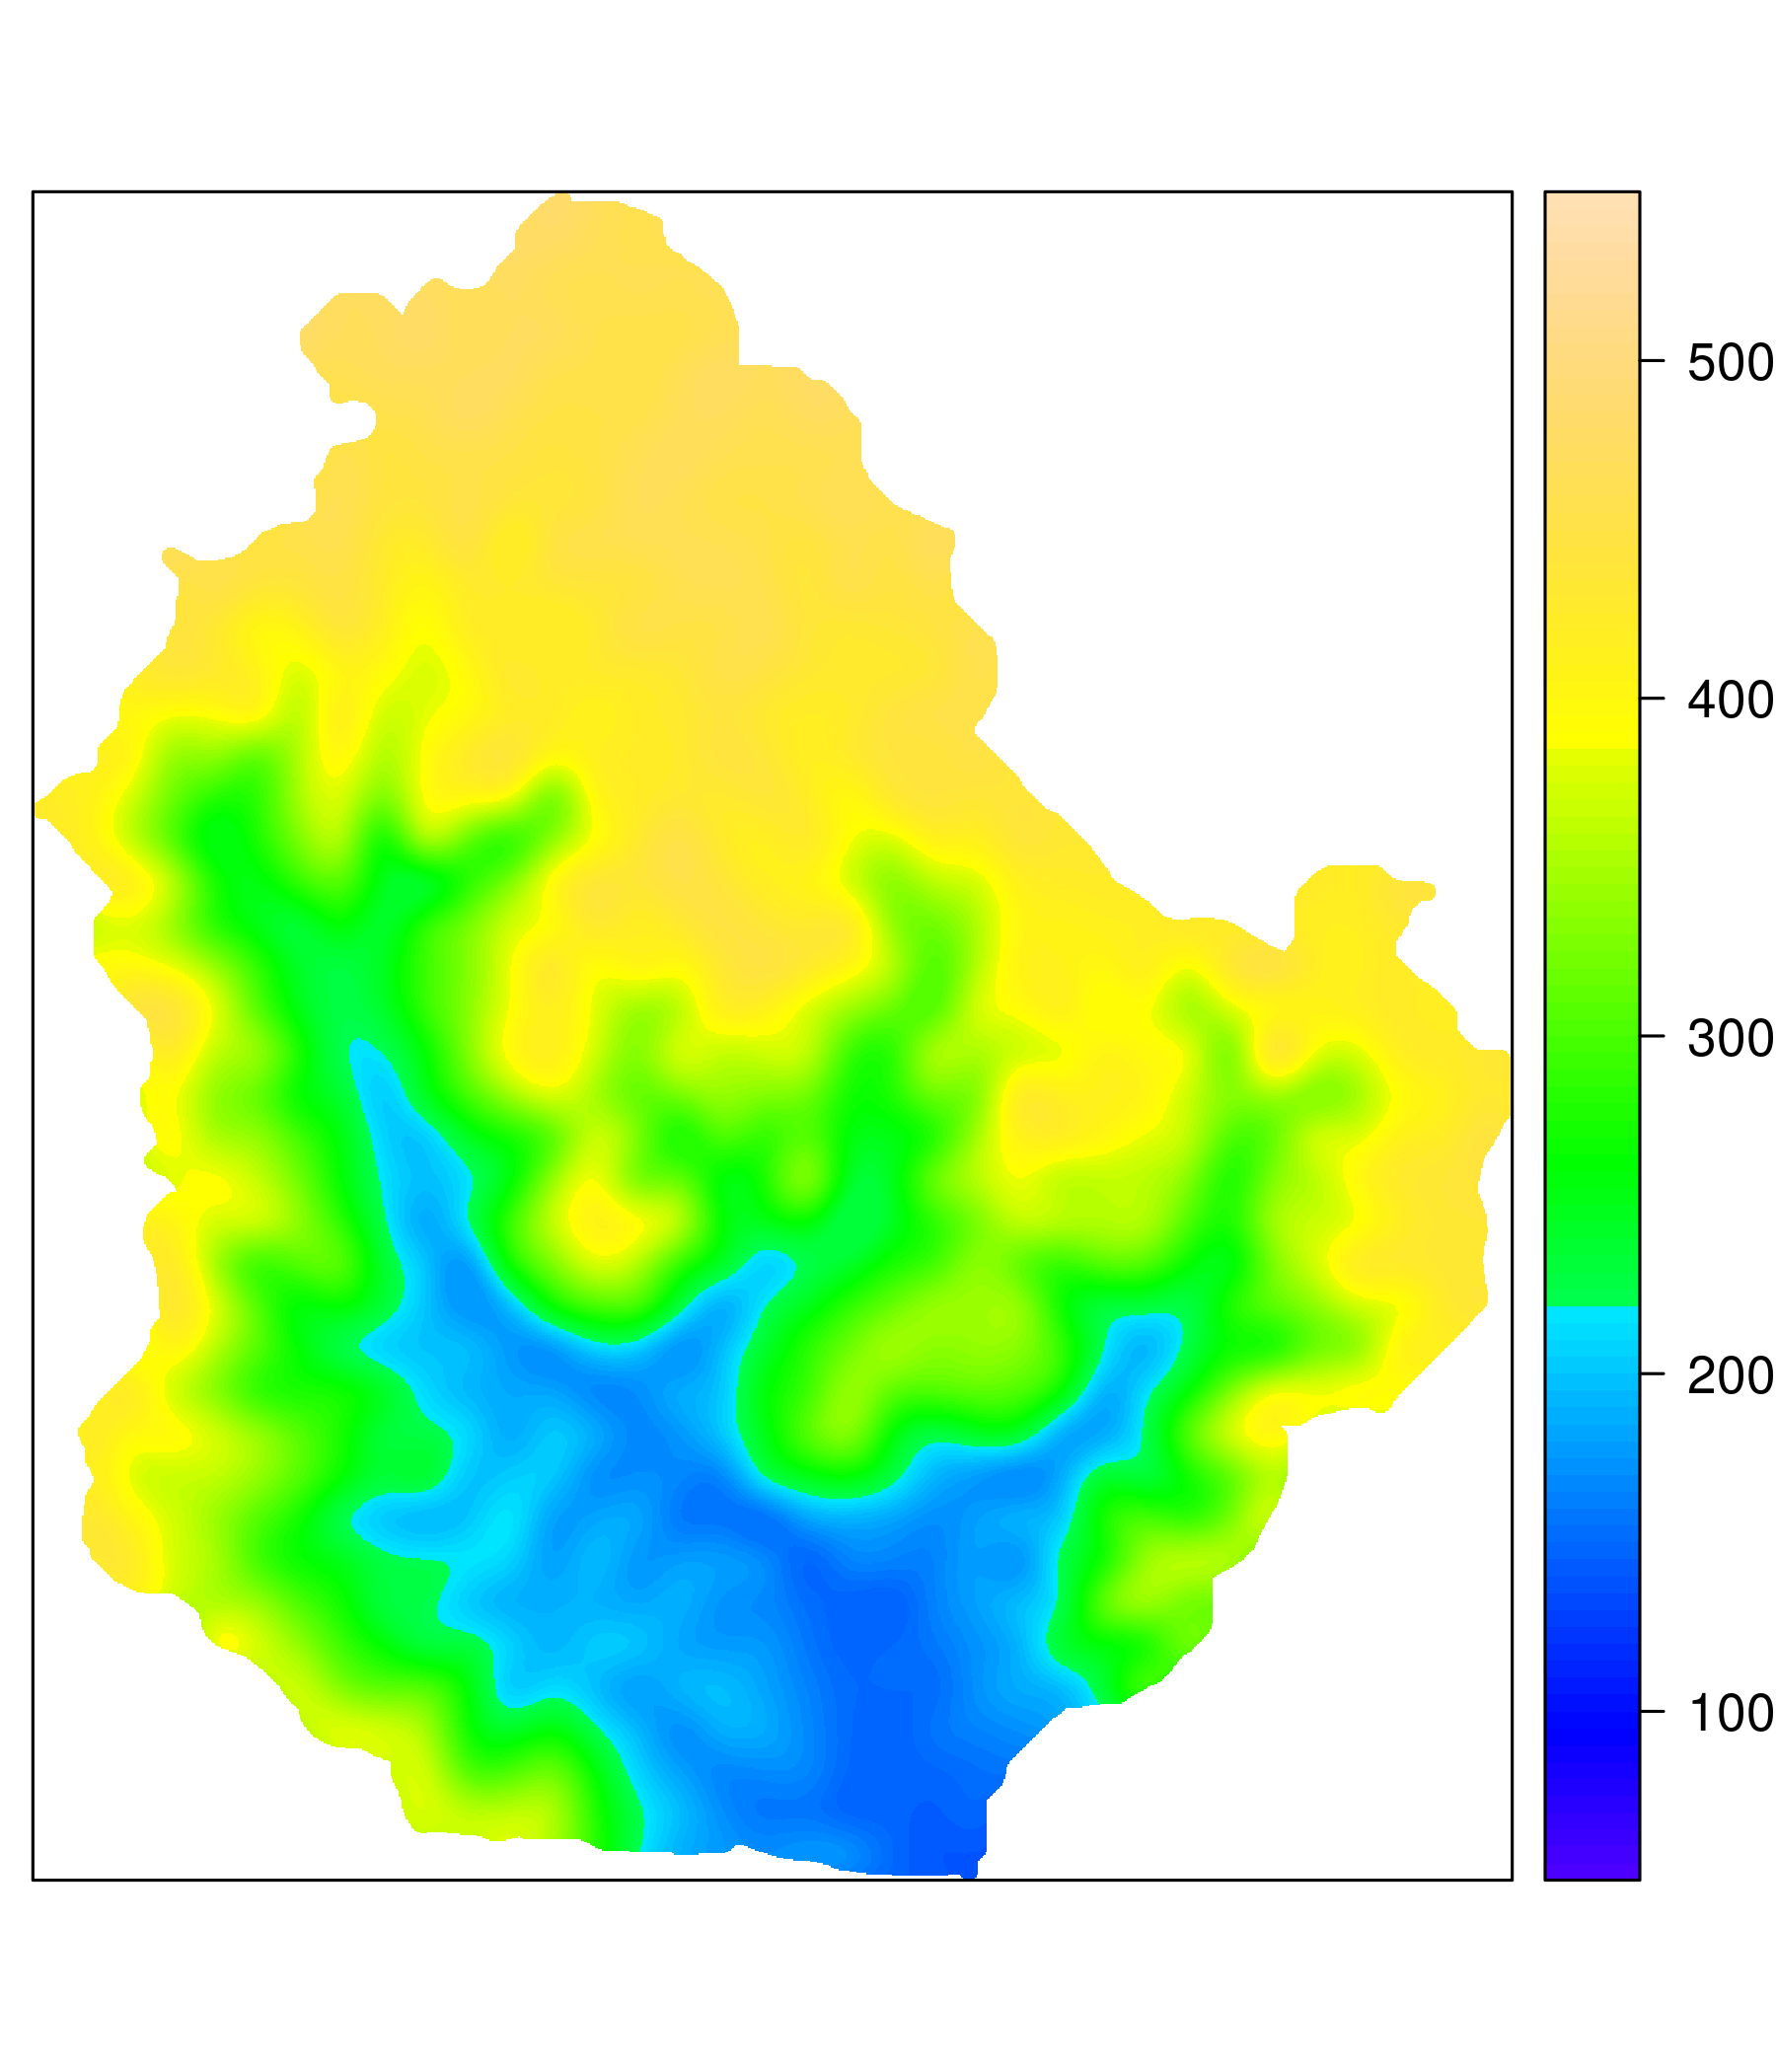
\includegraphics[width = \textwidth]{fig/chap05-dem-old}
\end{minipage}
\begin{minipage}[b]{0.45\textwidth}
\subcaption{}
\label{fig:chap05-dem-new}
\centering
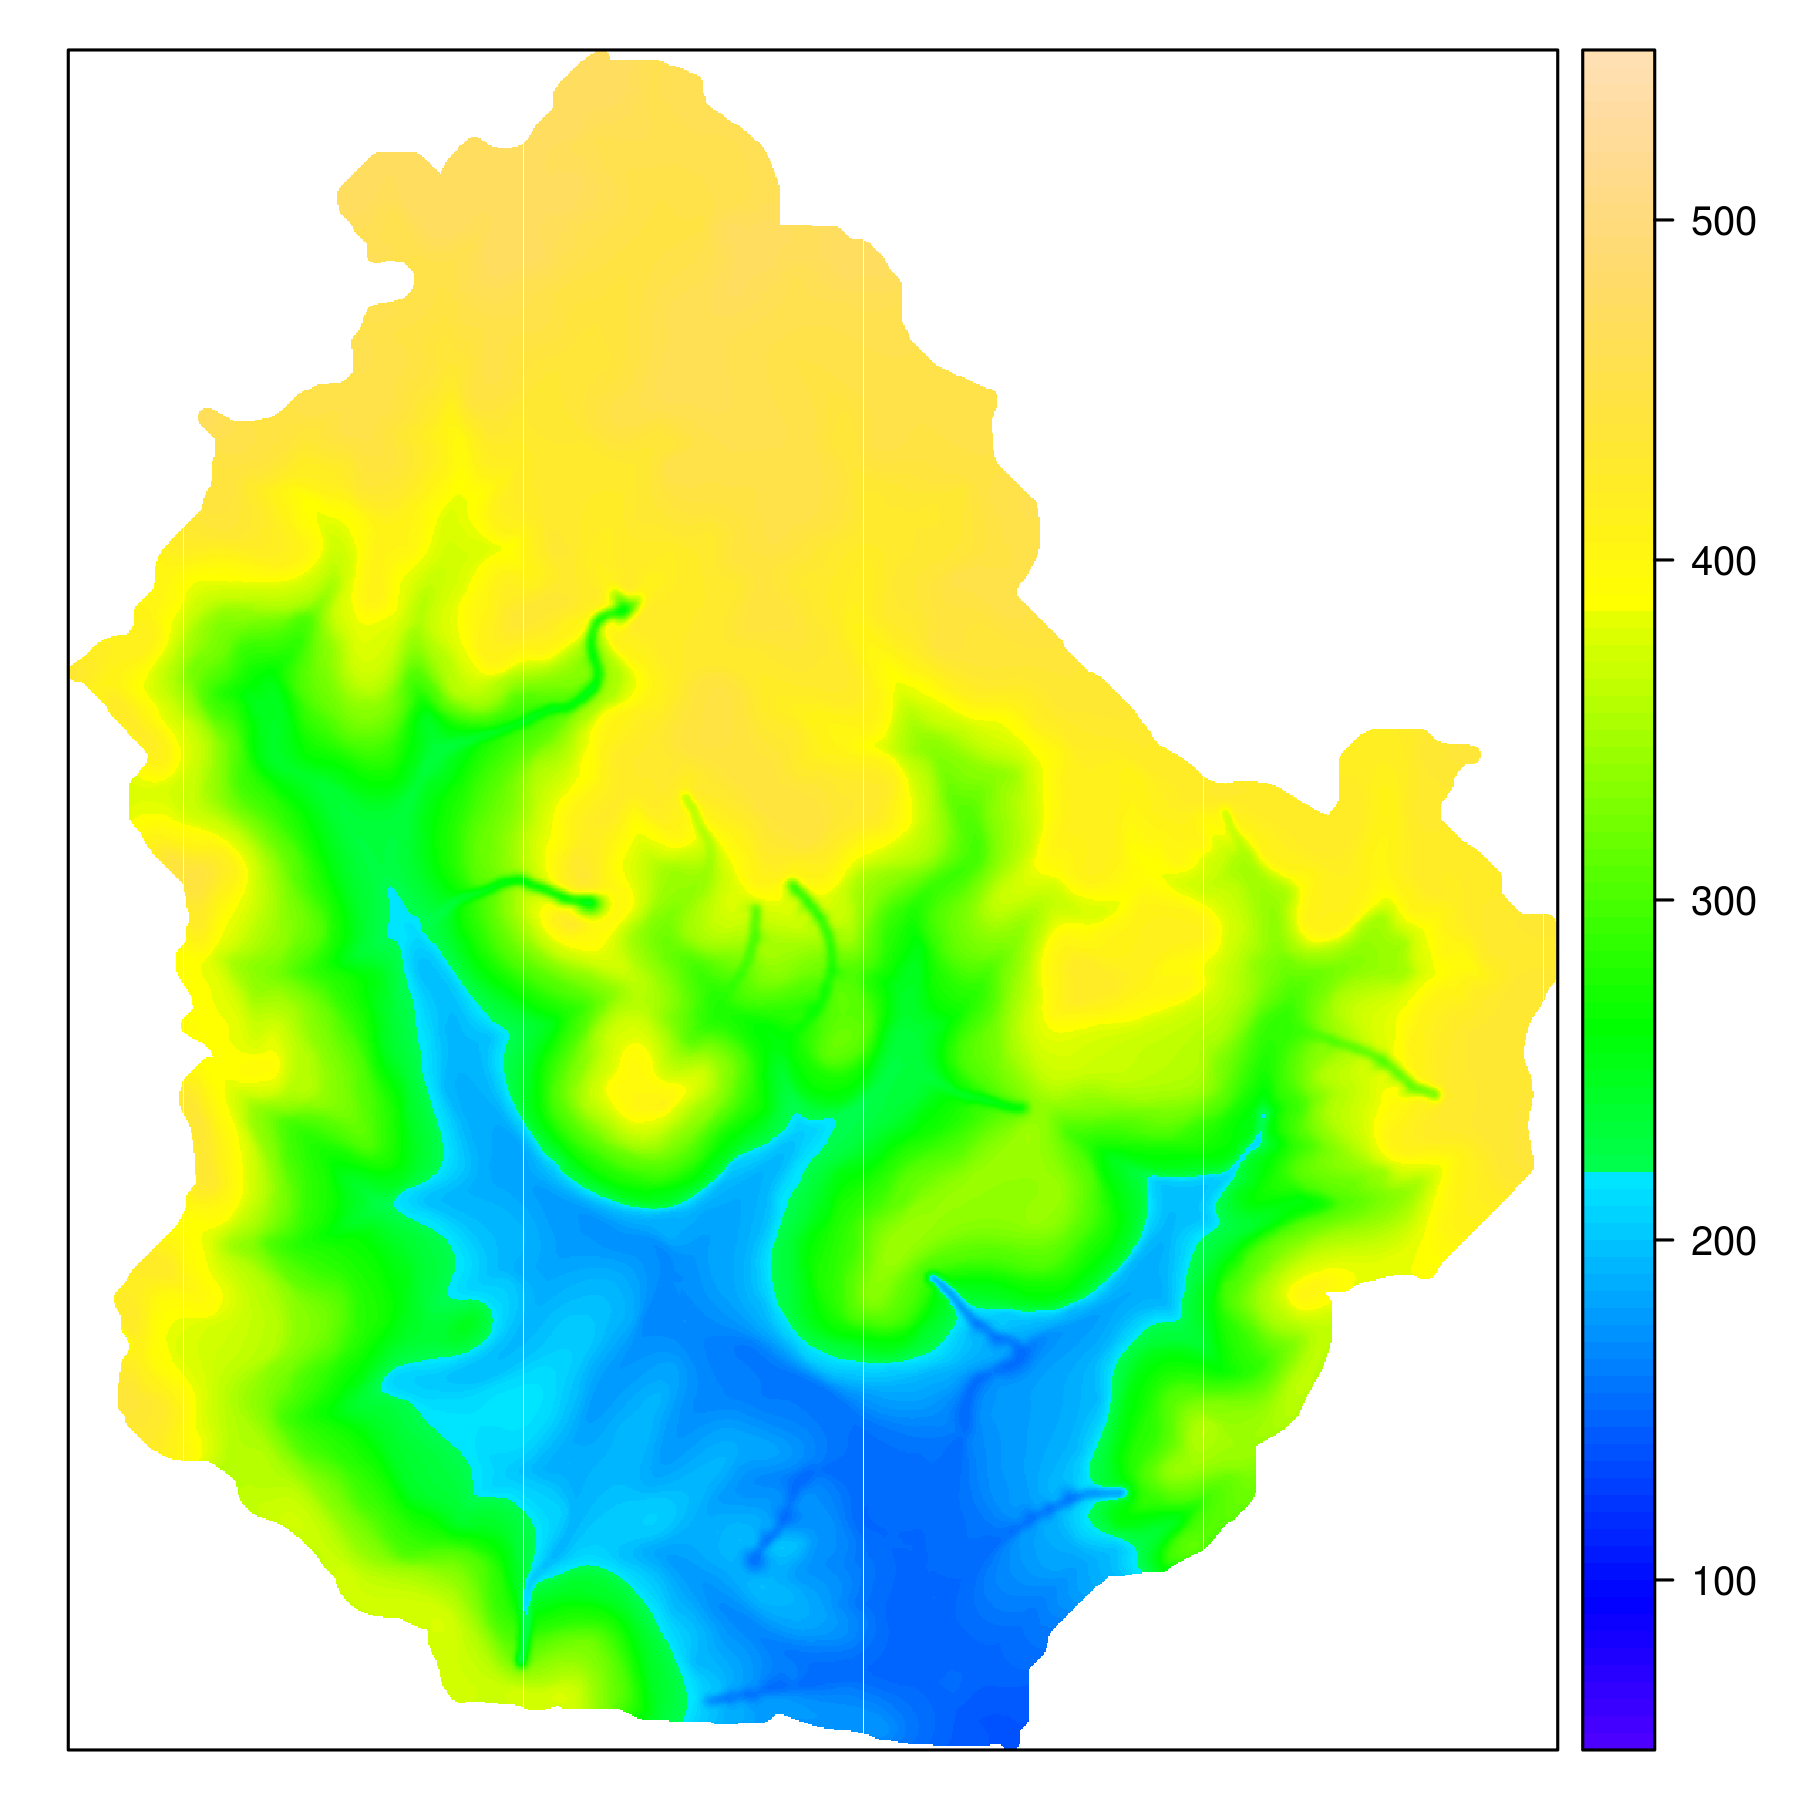
\includegraphics[width = \textwidth]{fig/chap05-dem-new}
\end{minipage} 
\caption[Digital elevation models included in the Santa Maria dataset.]{Digital elevation models (a) \demOld{} 
and (b) \demNew{} used to derive terrain covariates included in the Santa Maria dataset.}
\label{fig:chap05-dem}
\end{figure}

A third DEM (not shown) was included in the Santa Maria dataset with the sole purpose of supporting the 
orthorectification -- removal of the effects of the perspective of the sensor on the relative position of 
objects in the image -- and topographic correction -- removal of the effects of the topography on the 
reflectance values, i.e. on the illumination of the geomorphic surfaces -- of satellite images 
(\autoref{sec:chap05-sat-image}) \cite{Mather2004, Schowengerdt2007}. The third DEM (\topodata) was produced 
by the Brazilian National Institute for Space Research (\inpe) by refining the SRTM DEM version 1 
(\q{unfinished}) to $\SI{1}{\arcsecond} \approx \SI{30}{\m}$ spatial resolution using ordinary kriging with a 
Gaussian spatial autocorrelation model \cite{ValerianoEtAl2012}. Eight tiles were mosaicked 
(\gdal{gdal\_translate}) and the CRS transformed from WGS1984 (EPSG:4326) to WGS1984 / UTM zone 22S 
(EPSG:32722) using cubic resampling (\gdal{gdalwarp}), and the sinks filled using \grass{r.fill.dir}. Before 
the atmospheric correction of satellite images, orthometric heights were converted to ellipsoidal heights 
using \autoref{eqn:geoidal}, the geoidal undulation calculated with the gravitational model EGM1996. This 
conversion was done because orbital satellites use the WGS1984 ellipsoid as vertical datum. For the 
orthorectification of satellite images, the DEM was then processed using \grass{r.resamp.interp} with the 
bicubic resampling method to match the reference grid.

The three DEMs present similar vertical accuracy (\autoref{tab:chap05-dem-attr-val}). In the case of 
\demNew{}, which was derived from contour lines published at a \scale{25000}, the vertical positional accuracy 
does not meet the high-quality standards of current Brazilian legislation, which states that 
\SI{90}{\percent} of the GCPs should have vertical errors smaller than \SI{5}{\metre}, which is half of the 
distance between contour lines \cite{Brasil1984}. The corresponding RMSE should be less than \SI{3}{\metre}.

\ctable[
  caption  = {Error statistics of the vertical validation of \demOld, TOPODATA, and \demNew{} using $n = 60$
  validation points located along $m = 12$ linear transects.},
  cap      = {Error statistics of the vertical validation of \demOld, TOPODATA, and \demNew.},
  label    = tab:chap05-dem-attr-val,
  notespar,
  pos      = !ht,
  maxwidth = \textwidth,
  % doinside = \scriptsize\setstretch{1.1},
  doinside = \small
  ]{lrrrrrr}{
  }{                                                              \FL
  Statistics                   & \demOld{} & TOPODATA & \demNew{} \ML
  Mean, \si{\m}                & -15       & -17      & -16       \NN
  Absolute mean, \si{\m}       & 15        & 17       & 16        \NN
  Squared mean, \si{\m\square} & 350       & 361      & 374       \LL
  }

% Figure \ref{fig:cdf-elev} shows that estimated validation statistics have different cumulative 
% distribution functions (CDF). The estimates are more uniformly distributed along the interval of 
% values for \texttt{ELEV\_10} than for \texttt{ELEV\_90} and \texttt{ELEV\_30}. While 
% \texttt{ELEV\_10} has a 50\% probability that absolute errors are below 15 m, \texttt{ELEV\_90} has 
% a 70\% probability that absolute errors are below 15 m. This suggests that the accuracy of 
% \texttt{ELEV\_90} is very consistent across the study area, with a few extreme values, while the 
% accuracy of \texttt{ELEV\_10} have a stronger spatial variation. For \texttt{ELEV\_30}, the 
% interpolation method used to refine the original SRTM DEM to 30 m \cite{ValerianoEtAl2012} seems to 
% have produced a spatial redistribution of the errors.

% \begin{figure}[!ht]
%   \centering
%   \includegraphics[width=0.9\textwidth]{fig/cdf-ELEV-90} 
%   \includegraphics[width=0.9\textwidth]{fig/cdf-ELEV-30}
%   \includegraphics[width=0.9\textwidth]{fig/cdf-ELEV-10}
%   \caption{Cumulative distribution functions of mean error, mean absolute error, and squared error of 
% elevation values estimates by digital elevation models \texttt{ELEV\_90}, \texttt{ELEV\_30}, and 
% \texttt{ELEV\_10}.}
%   \label{fig:cdf-elev}
% \end{figure}

Despite all DEMs present a similar vertical accuracy, \demNew{} is considered the highest quality DEM in the 
Santa Maria dataset. Because it was produced using information about the drainage network and location of 
lakes and natural depressions, it is likely to provide a better hydrological representation of the DNOS 
catchment. As such, \demNew{} was used to estimate the geographical limits (boundary) of the DNOS catchment, 
for which GRASS GIS modules \texttt{r.watershed} and \texttt{r.water.outlet} were employed. Because the 
overall deviation between the affine-corrected coordinates of topographic maps and target coordinates of GCPs 
is $\text{RMSE} = \SI{29.55}{\m}$ -- there still is uncertainty about the correct position of topographic maps 
-- a \SI{30}{\m} buffer was added to the estimated geographical limits of the DNOS catchment. The water outlet 
point used to estimate the boundary is located on the bridge that crosses the main drainage channel 
(\ang{-29.65868}, \ang{-53.78969}).

Eight terrain attributes were derived from each of \demOld{} and \demNew{} to produce the covariate data 
included in the Santa Maria dataset, the first of them being elevation (\texttt{ELEV}). The others are slope, 
aspect, northernness, flow accumulation, topographic wetness index, stream power index, and topographic 
position index.

Slope (\texttt{SLP}) and aspect (\texttt{ASP}) were calculated using \grass{r.param.scale}. This module 
calculates terrain attributes by fitting a bivariate quadratic polynomial using least squares \cite{Wood1996}. 
It allows using different window sizes to fit the bivariate quadratic polynomial, thus including the effect of 
scale in the calculation of terrain attributes. Seven window sizes were used (3, 7, 15, 31, 63, 127, and 255) 
and the results for calculated slope can be seen in \autoref{fig:chap05-slope}. Larger window sizes result in 
a smoother version of the terrain attribute, while smaller windows sizes result in raster maps with more 
(small-scale) details. Several flat surfaces (slope of \ang{0}) were produced in the slope raster maps 
calculated using \texttt{ELEV\_90} as a result of resampling the original DEM from \num{90} to \SI{5}{\m}. A 
value of \ang{0.1} was added to the rasters to remove these flat surfaces.

\begin{figure}[!ht]
\centering
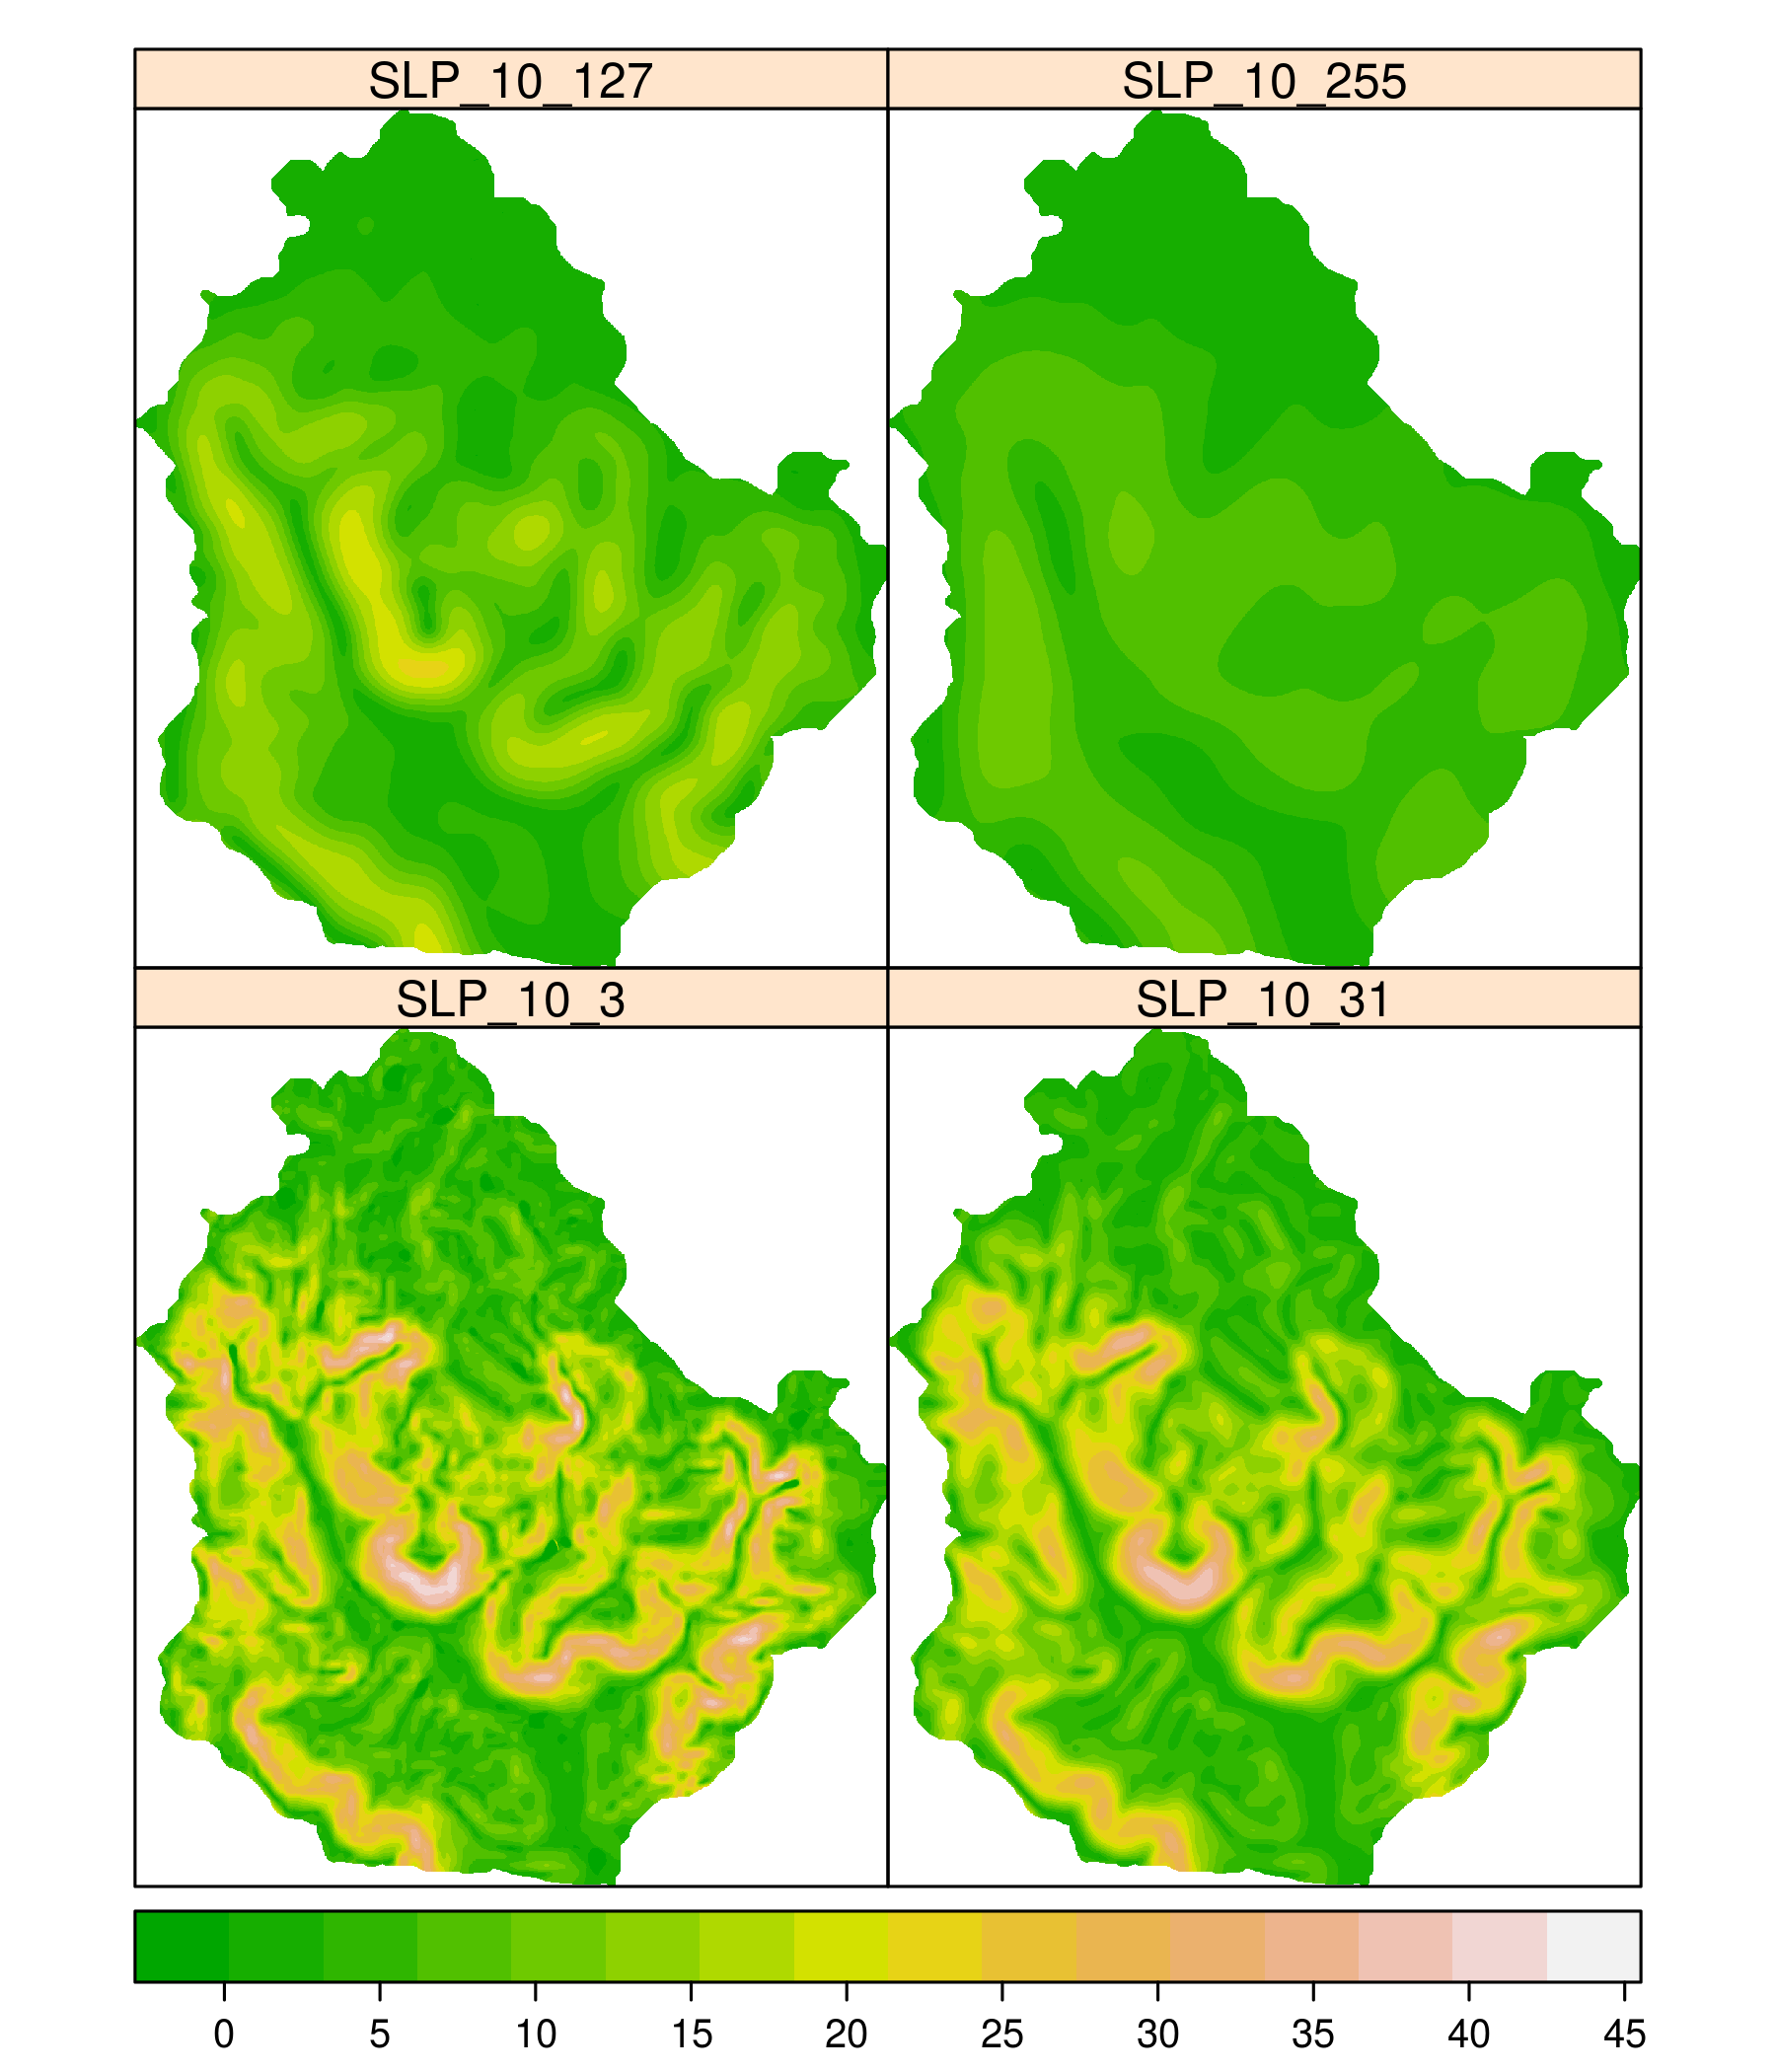
\includegraphics[width = 0.90\textwidth]{fig/chap05-slope}
\caption[Slope derived using windows of different sizes.]{Slope \texttt{SLP} raster surfaces derived from 
\demNew{} using windows of sizes (from left to right) $3 \times 3$, $31 \times 31$, $127 \times 127$, and $255 
\times 255$.}
\label{fig:chap05-slope}
\end{figure}

Aspect values had to be corrected before use because \grass{r.param.scale} stores aspect values in the range 
0--\SI{+180}{\degree} from West to North to East, and 0--\SI{-180}{\degree} from West to South to East, when 
the standard procedure is to work with aspect values ranging from 0--\SI{360}{\degree} clockwise. This 
correction was done using

\begin{equation}
 \texttt{ASP}_{0} =
 \begin{cases}
  \texttt{ASP}_{GRASS} + \ang{360} & \text{if}\;\; \texttt{ASP}_{GRASS} < \ang{0}, \\
  \texttt{ASP}_{GRASS}             & \text{else},
 \end{cases}
\end{equation}

\noindent and

\begin{equation}
 \texttt{ASP} =
 \begin{cases}
  \texttt{ASP}_{0} + \ang{270} & \text{if}\;\; \texttt{ASP}_{0} < \ang{90}, \\
  \texttt{ASP}_{0} - \ang{90}  & \text{else}.
 \end{cases}
\end{equation}

\noindent A second correction of aspect values involved their linearisation. This is necessary because aspect 
is a circular variable, that is, the beginning (\ang{0}) and end (\ang{360}) of the measurement scale have the 
same physical meaning. Aspect values were transformed to northernness (\texttt{NOR}), a measure of the level 
of exposition of a given surface to the North, a linear variable, using the equation

\begin{equation}\label{eqn:NOR}
 \texttt{NOR} = abs(\ang{180} - \texttt{ASP}).
\end{equation}  

Flow accumulation (ACC), also known as catchment area or contributing area, was calculated using 
\grass{r.watershed}, the resulting raster surface being multiplied by the square of the cell size (i.e. by the 
cell area \SI{25}{\metre\square}) to convert to areal units. This raster surface was used to calculate 
the topographic wetness index (\texttt{TWI}) and the stream power index (\texttt{SPI}) using

\begin{equation}\label{eqn:sACC}
 \text{sACC} = \dfrac{\text{ACC}}{5},
\end{equation}

\begin{equation}\label{eqn:TWI}
 \texttt{TWI} = log \dfrac{\text{sACC}}{tan(\texttt{SLP})},
\end{equation}

\noindent and

\begin{equation}\label{eqn:SPI}
 \texttt{SPI} = log(\text{sACC} \times tan(\texttt{SLP})),
\end{equation}

\noindent where sACC is the specific catchment area, \SI{5}{\m} is the cell size, and \texttt{SLP} is the 
slope raster surface calculated using seven different window sizes.

The topographic position index \texttt{TPI} was calculated with \saga{ta\_morphometry}. Different values of 
maximum radius were used to include the effect of scale, all of them related to the window sizes used to 
calculate previous terrain attributes. A minimum radius value of \SI{3}{\m} was used in all calculations.

A total of $p = 1 \times \texttt{ELEV} + 7 \times (\texttt{NOR}, \texttt{SLP}, \texttt{TWI}, \texttt{SPI}, 
\texttt{TPI}) = 36$ covariates were defined using the terrain attributes derived from \demOld{} and \demNew{}.

\section{GEOLOGIC MAPS}
\label{sec:chap05-geo-maps}

Geologic data comes from the two most recent geologic maps (\geoOld{} -- \autoref{fig:chap05-geo-old}, and 
\geoNew{} -- \autoref{fig:chap05-geo-new}) published at the \scales{50000}{25000} \cite{GasparettoEtAl1988, 
MacielFilho1990}. Both of them were produced based on the most recent topographic sheets produced by the 
Brazilian Army at the \scales{50000}{25000} \cite{DSG1980, DSG1992, DSG1992a}. Alike topographic maps, 
geologic maps were available only in analogical format, and were hand digitized and georeferenced in QGIS. 
Intersections between all meridians and parallels ($n = 16$) were used as control points to adjust a second 
order polynomial model. Resampling was performed using the cubic resampling method. The original CRS 
(EPSG:31982 -- SIRGAS2000 / UTM zone 22S) was transformed to match the reference grid using the 
\Rpackage{rgdal} \cite{BivandEtAl2013a}.

\begin{figure}[!ht]
\centering
\begin{minipage}[b]{0.45\textwidth}
\subcaption{}
\label{fig:chap05-geo-old}
\centering
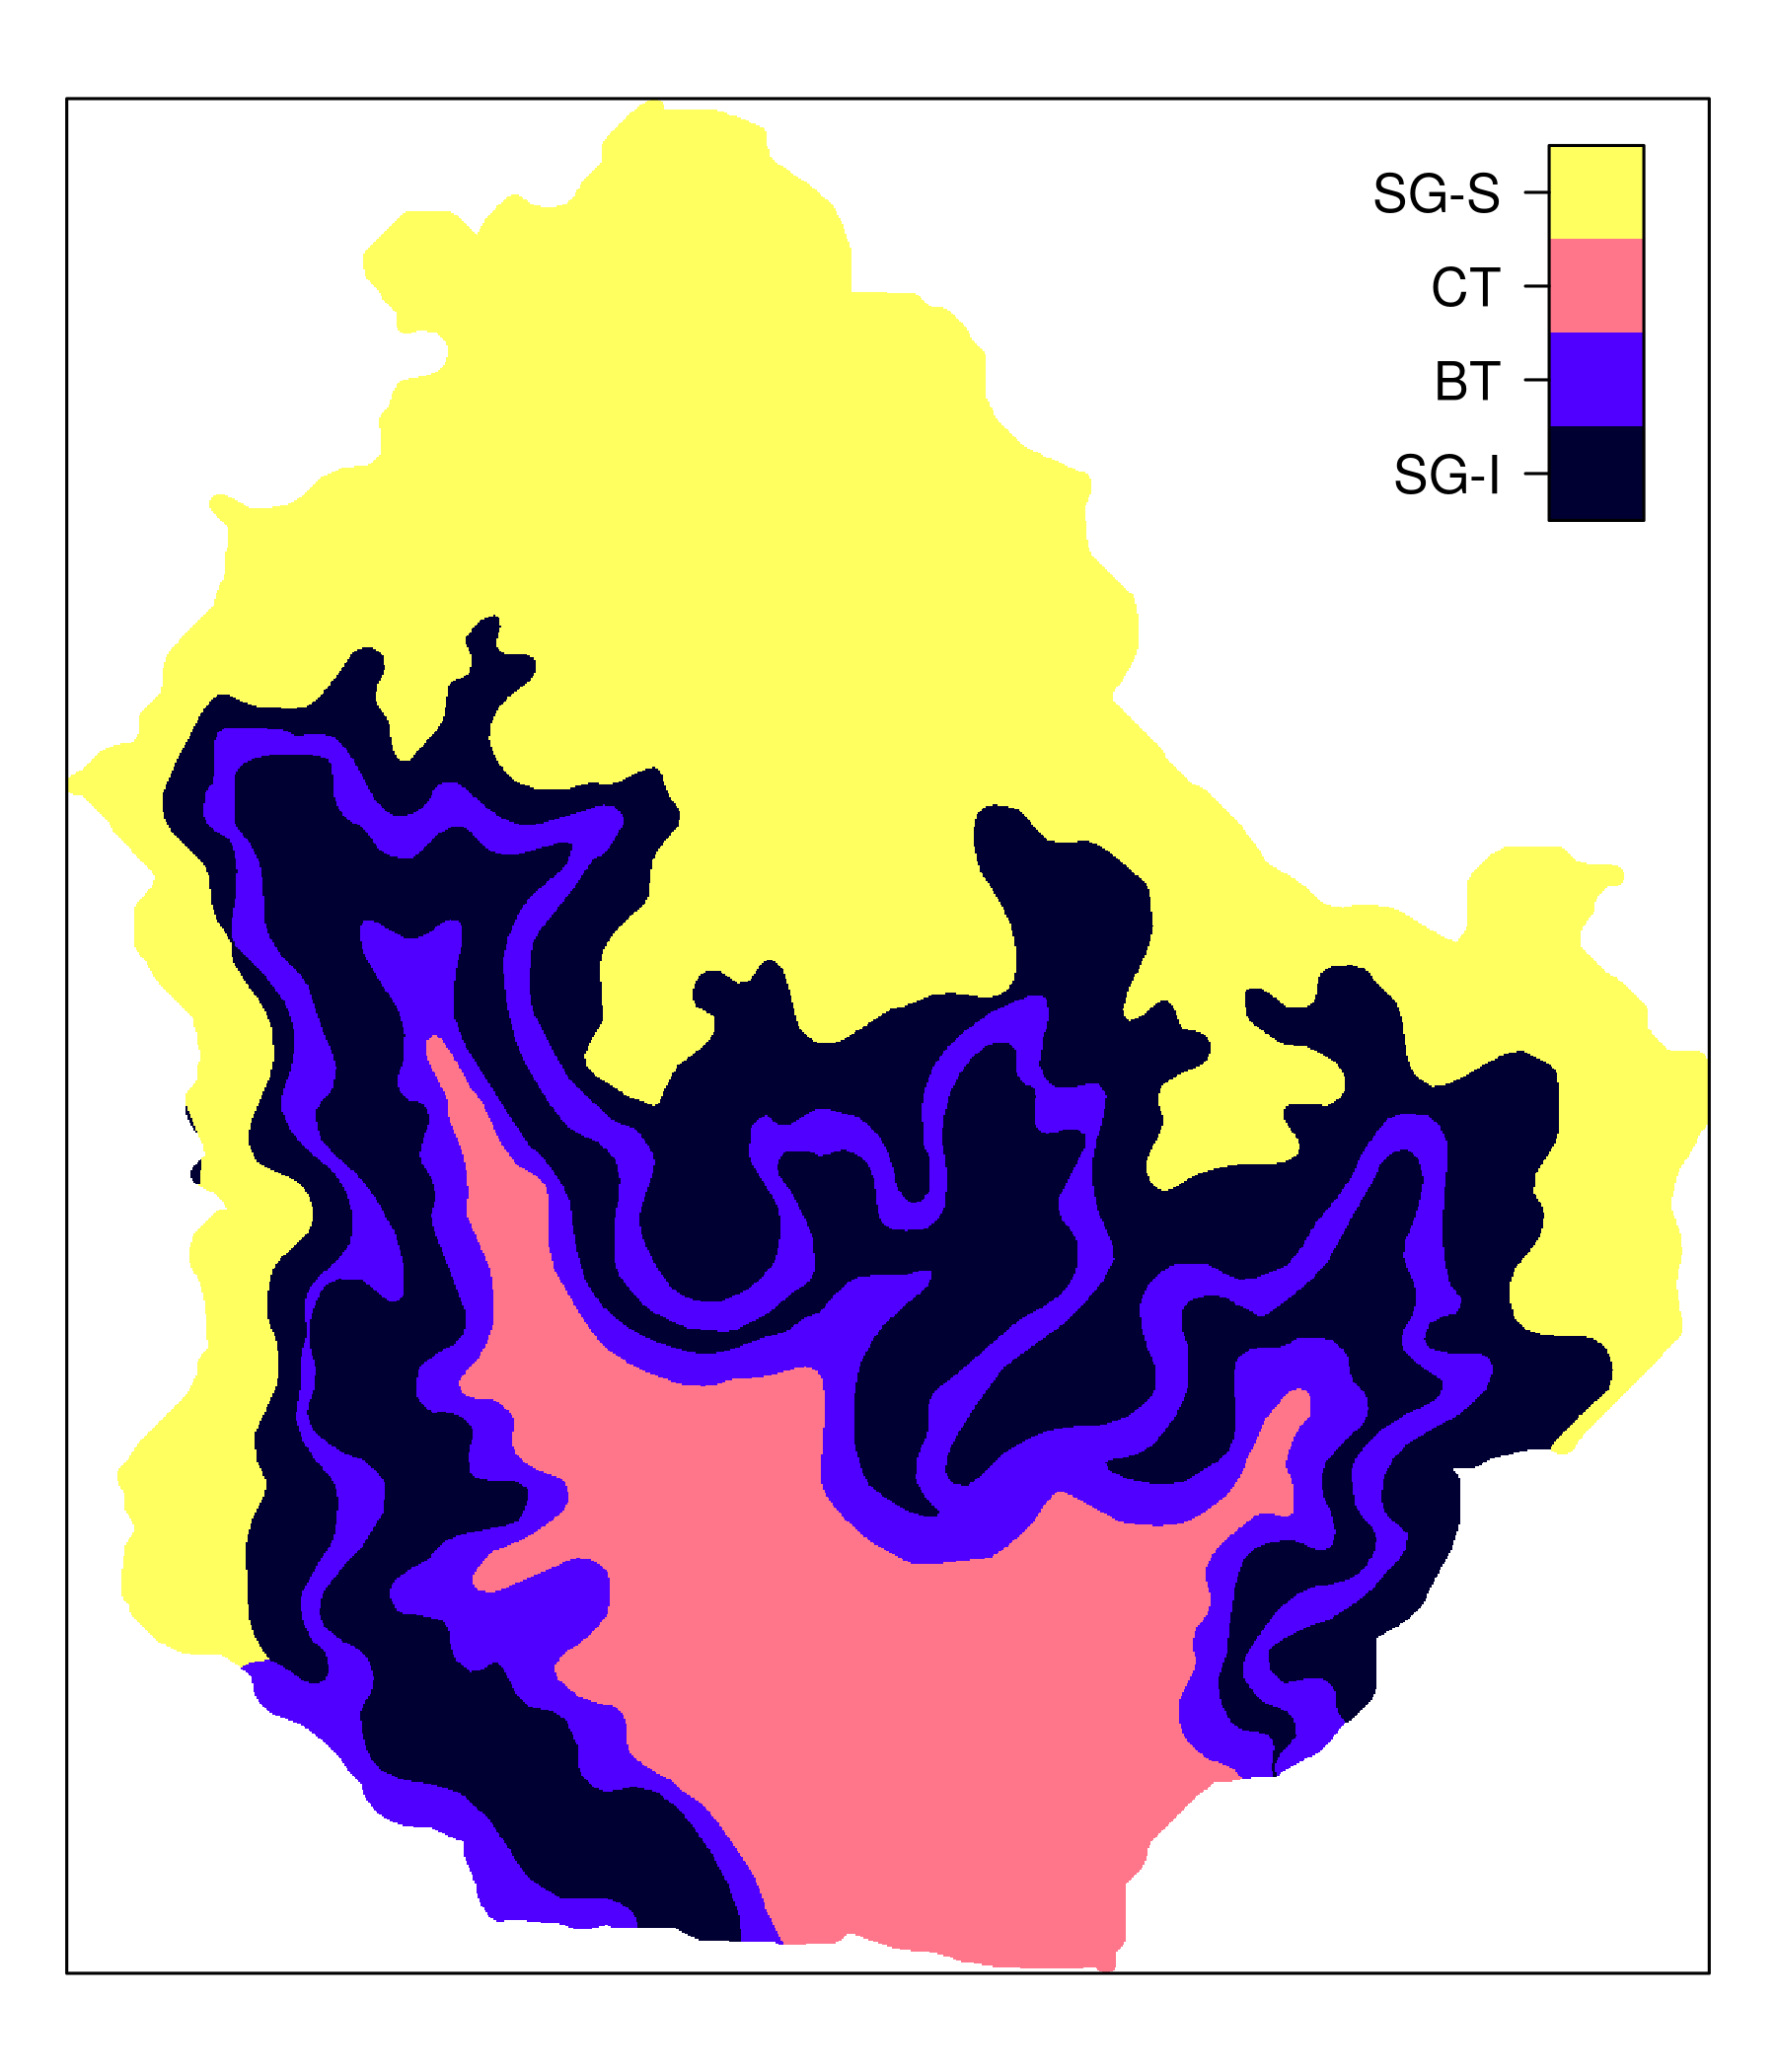
\includegraphics[width = \textwidth]{fig/chap05-geo-old}
\end{minipage}
\begin{minipage}[b]{0.45\textwidth}
\subcaption{}
\label{fig:chap05-geo-new}
\centering
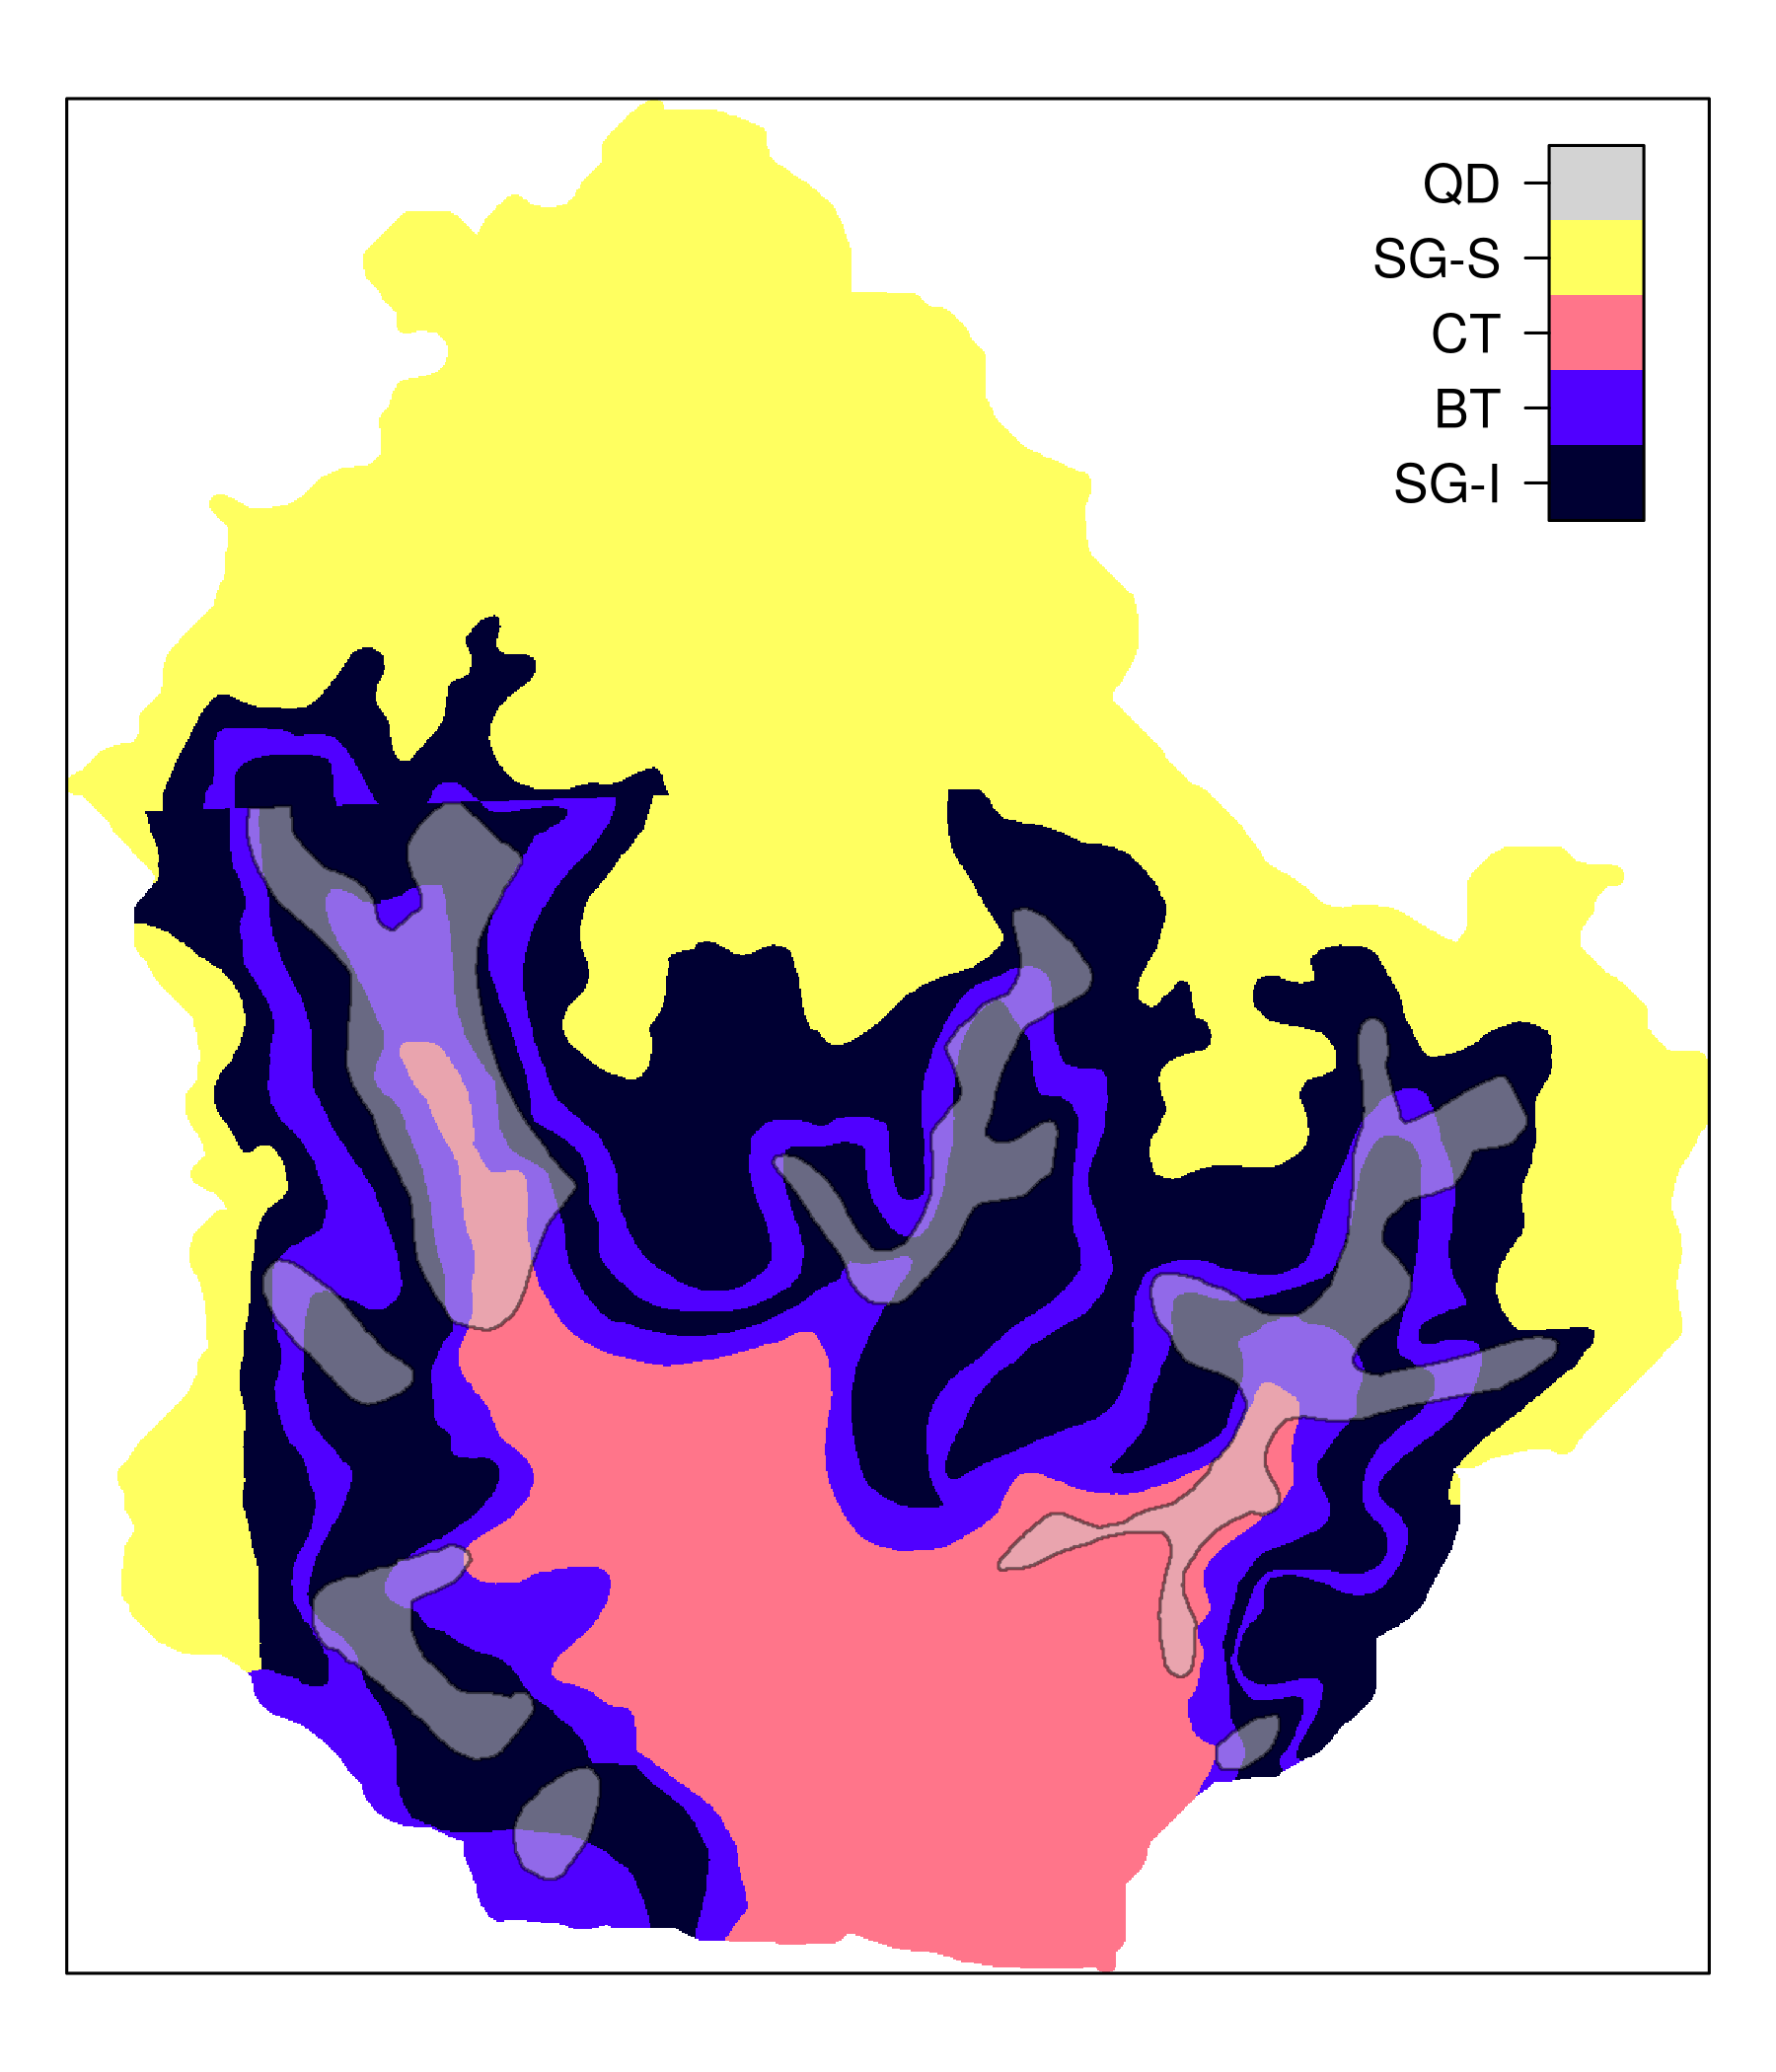
\includegraphics[width = \textwidth]{fig/chap05-geo-new}
\end{minipage} 
\caption[Geologic maps included in the Santa Maria dataset.]{Geologic maps (a) \geoOld{} and (b) \geoNew{} 
used to derive indicator covariates included in the Santa Maria dataset. Legend abbreviations and derived 
indicator variables are described in the text.}
\label{fig:chap05-geo-maps}
\end{figure}

The positional validation of geologic maps was performed using $n = 8$ (\geoOld{}) and $n = 5$ (\geoNew{}) 
GCPs, respectively. Validation statistics show that the positional accuracy of neither geologic maps meets the 
high-quality standards of the current Brazilian legislation (\autoref{tab:chap05-geology-geo-val}). Estimated 
RMSE are \num{147} and \SI{69}{\m} for \geoOld{} and \geoNew{}, respectively, when the maximum RMSE 
recommended are \num{25} and \SI{13}{\m}, respectively. For \geoOld{}, the lowest accuracy is found in the 
y-coordinate, while for \geoNew{}, the x-coordinate is the least accurate. Validation statistics suggest that 
there is a strong systematic error, which probably was propagated from the topographic maps used to produce 
the geologic maps. Therefore, the same strategy (affine transformation) used to remove the systematic 
positional error of the topographic maps was employed on geologic maps. Due to the lack of GCPs, model 
parameters were adjusted using the same set of GCPs used for the validation. The estimated uncertainty (RMSE) 
of the affine transformation is \num{86} and \SI{22}{\m} for \geoOld{} and \geoNew{}, respectively.

\ctable[
  caption  = {Error statistics of the horizontal validation of geologic maps \geoOld{} and \geoNew{} using 
  $n = 8$ and $n = 5$ ground control points.},
  cap      = {Error statistics of the horizontal validation of geologic maps.},
  label    = tab:chap05-geology-geo-val,
  notespar,
  pos      = !ht,
  maxwidth = \textwidth,
  % doinside = \scriptsize\setstretch{1.1},
  doinside = \small
  ]{lrrrr}{
  }{                                                                          \FL
  Statistics                   & x-coord & y-coord & Error vector & Azimuth   \ML
  \multicolumn{5}{l}{\geoOld{} ($n = 8$)}                                     \ML
  Mean, \si{\m}                & 10      & -102    & 140          & \ang{169} \NN
  Absolute mean, \si{\m}       & 43      & 125     & -            & -         \NN
  Squared mean, \si{\m\square} & 3431    & 18067   & 21498        & -         \ML
  \multicolumn{5}{l}{\geoNew{} ($n = 5$)}                                     \ML
  Mean, \si{\m}                & 51      & 29      & 67           & \ang{58}  \NN
  Absolute mean, \si{\m}       & 51      & 29      & -            & -         \NN
  Squared mean, \si{\m\square} & 3457    & 1312    & 4769         & -         \LL
  }

% \begin{figure}[ht]
%  \centering
%  \caption{Histogram of the azimuth distribution of the validation of geologic maps 
%  \texttt{GEO\_50} (left) and \texttt{GEO\_25} (right) in the geographic space. Azimuth values were 
%  estimated using, respectively, eight and five ground control points located in easily identifiable 
% geographical 
%  markers. The graph was produced using \Rpackage{VecStatGraphs2D}.}
%  \label{fig:chap05-geology-azim}
% \end{figure}

Three ($p = 3$) indicator covariates were derived from \geoOld{}:

\begin{description}
\item[\texttt{GEO\_50a}] Inferior Sequence of the Serra Geral Formation. Composed mainly by basic igneous 
rocks (tholeiitic basalt and andesite). It is likely related to high soil clay content and effective cation 
exchange capacity.
 
\item[\texttt{GEO\_50b}] Superior Sequence of the Serra Geral Formation. Composed mainly by acid igneous rocks 
(granophyric rhyolite and rhyodacite). It is likely related to moderate to high \texttt{CLAY} and 
\texttt{ECEC}.
 
\item[\texttt{GEO\_50c}] Botucatu Formation. Composed mainly by aeolian sandstones. It is likely related to 
low \texttt{CLAY} and \texttt{ECEC}.
\end{description}

Four ($p = 4$) indicator covariates were derived from \geoNew{}, the first three of them having the same 
meaning of those derived from \geoOld{}:

\begin{description}
\item[\texttt{GEO\_25a}] Inferior Sequence of the Serra Geral Formation.
 
\item[\texttt{GEO\_25b}] Superior Sequence of the Serra Geral Formation.
 
\item[\texttt{GEO\_25c}] Botucatu Formation.
 
\item[\texttt{GEO\_25d}] Quaternary deposits of fluvial, alluvial, and colluvial origin. It can help 
explaining the low clay content in areas where the soil is believed to have developed from igneous rocks as 
depicted in less detailed geologic maps.
\end{description}

\section{LAND USE MAPS}
\label{sec:chap05-land-use}

The first land use map used to derive covariate data included in the Santa Maria dataset was produced by 
manually digitizing land use data of \num{1980} (\landOld{}, \autoref{fig:chap05-land-use-old}) published in 
the most recent topographic map produced by the Brazilian Army (\scale{25000}) \cite{DSG1992a, DSG1992}. Most 
processing steps, including the correction of positional bias, are described in \autoref{sec:chap05-dem}, 
except for the use of the nearest neighbour resampling method to match \landOld{} to the reference grid.

\begin{figure}[!ht]
\centering
\begin{minipage}[b]{0.45\textwidth}
\subcaption{}
\label{fig:chap05-land-use-old}
\centering
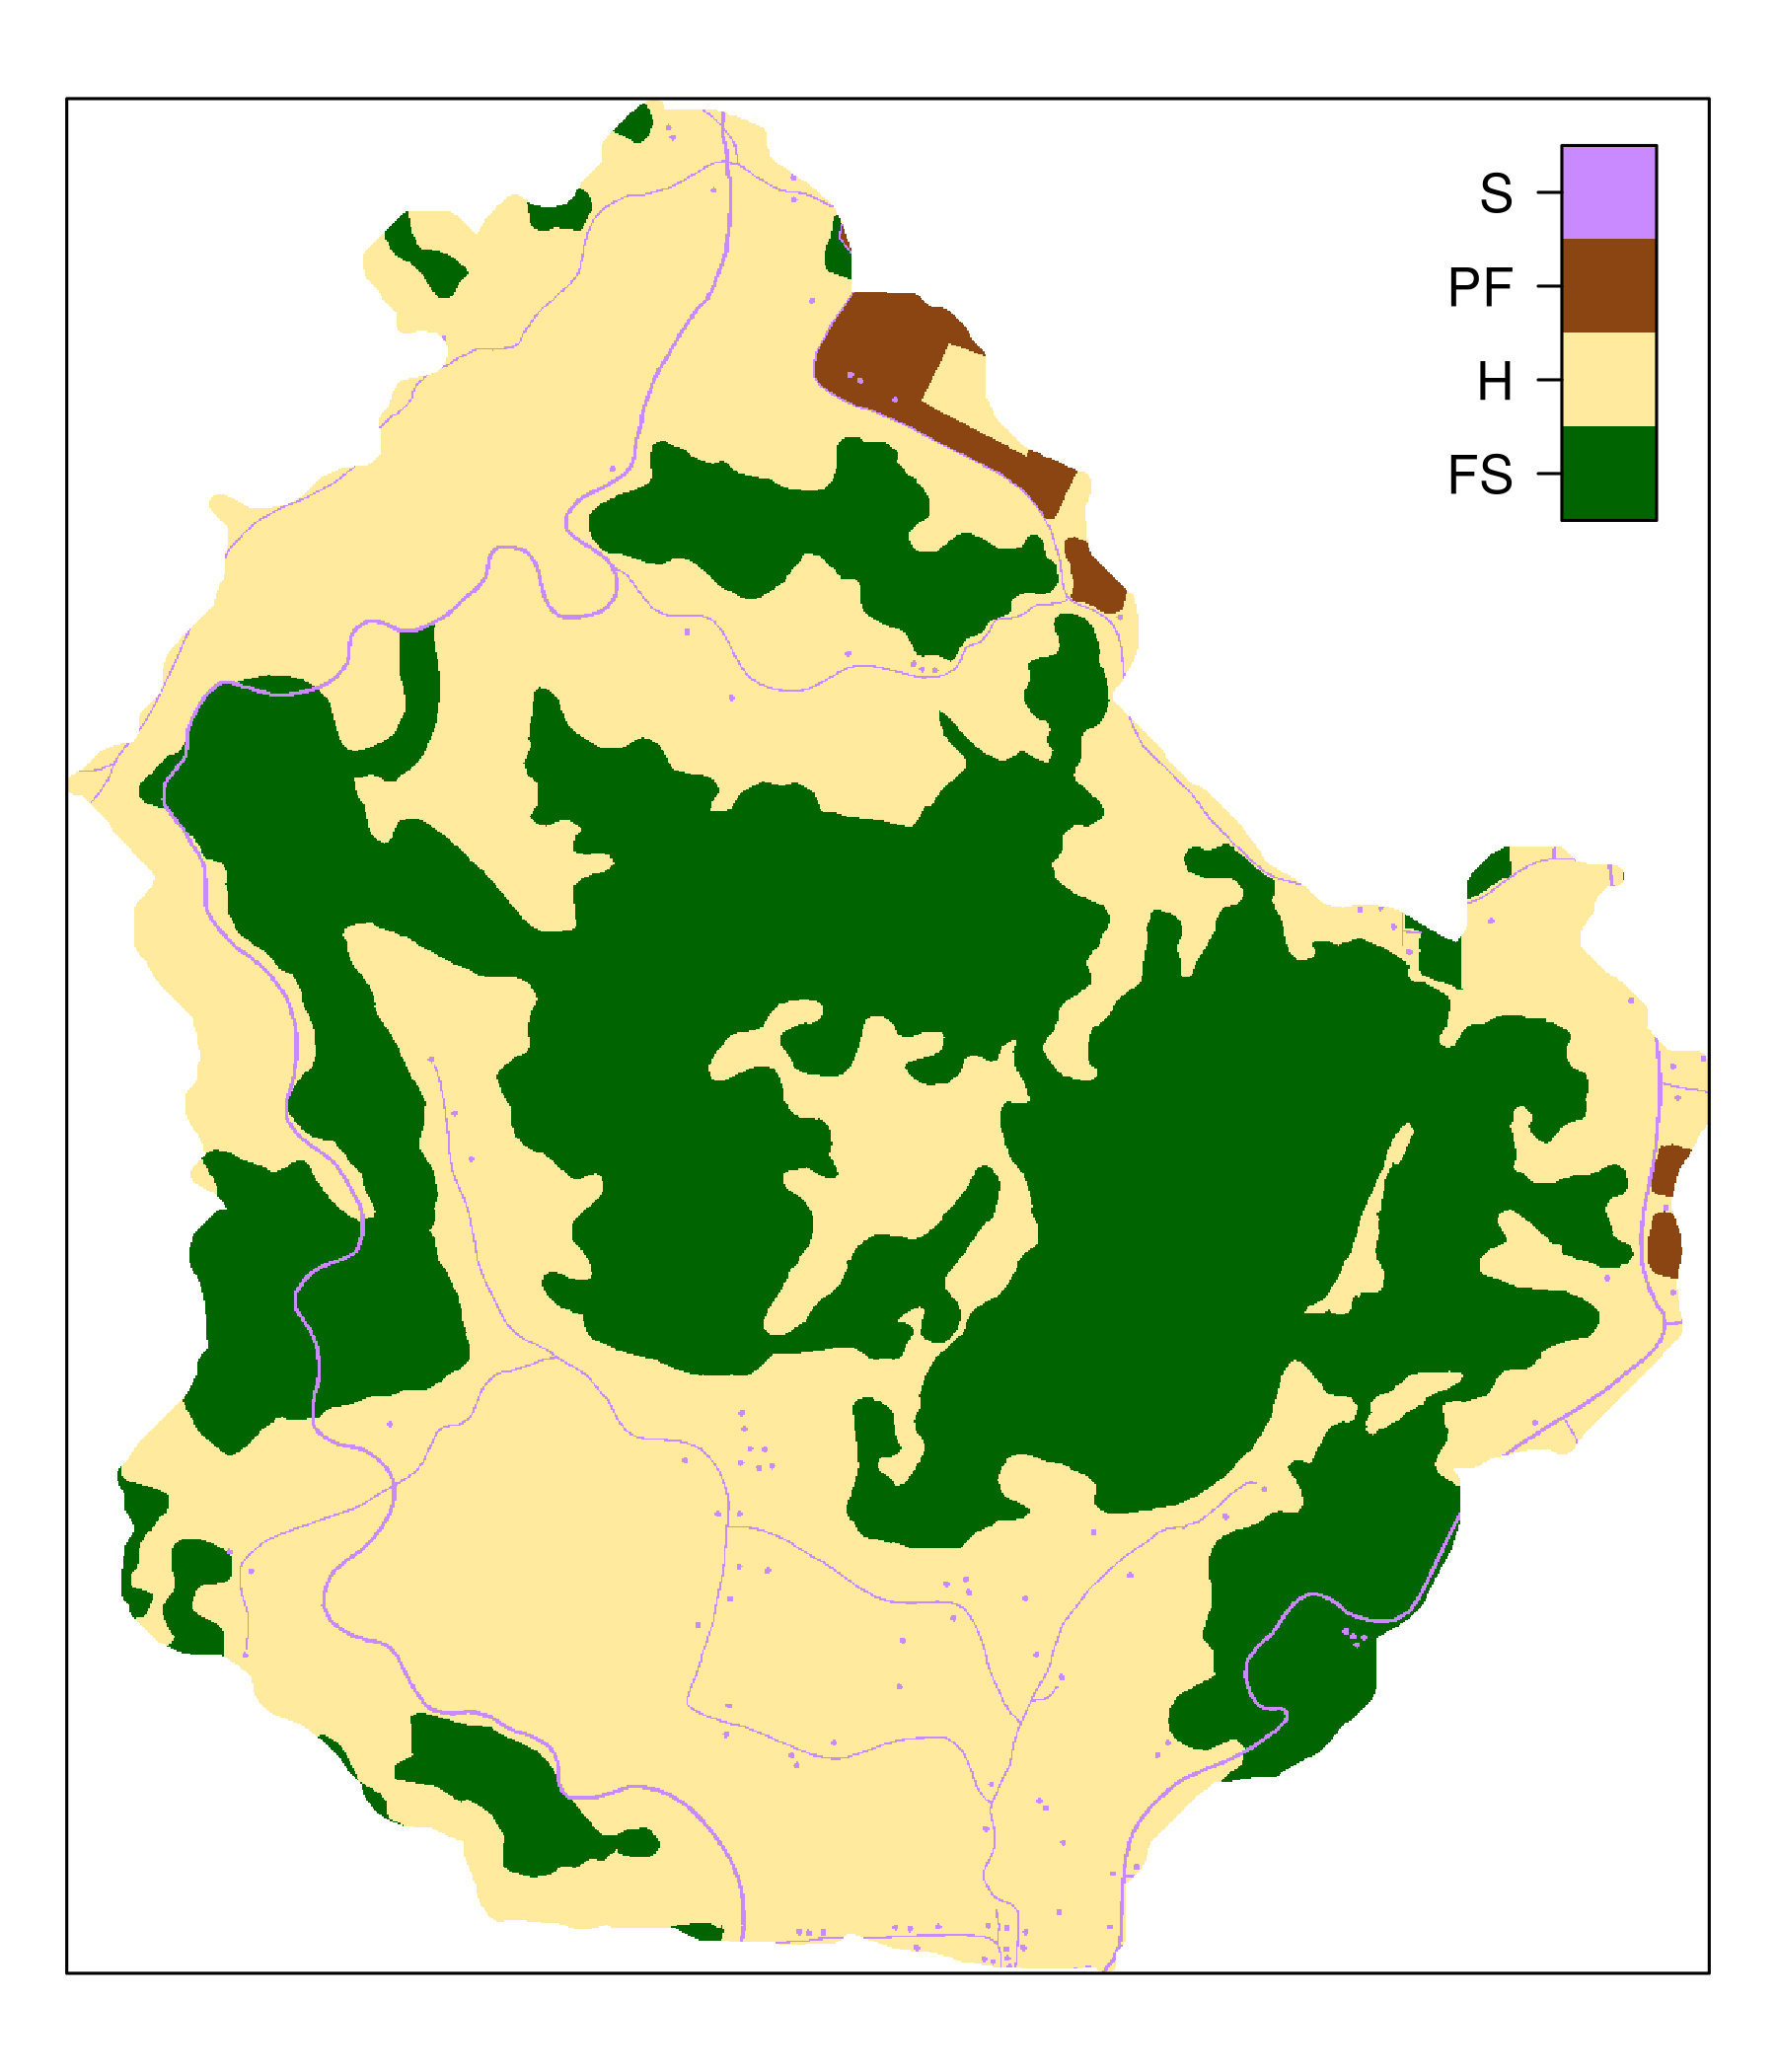
\includegraphics[width = \textwidth]{fig/chap05-land-old}
\end{minipage}
\begin{minipage}[b]{0.45\textwidth}
\subcaption{}
\label{fig:chap05-land-use-new}
\centering
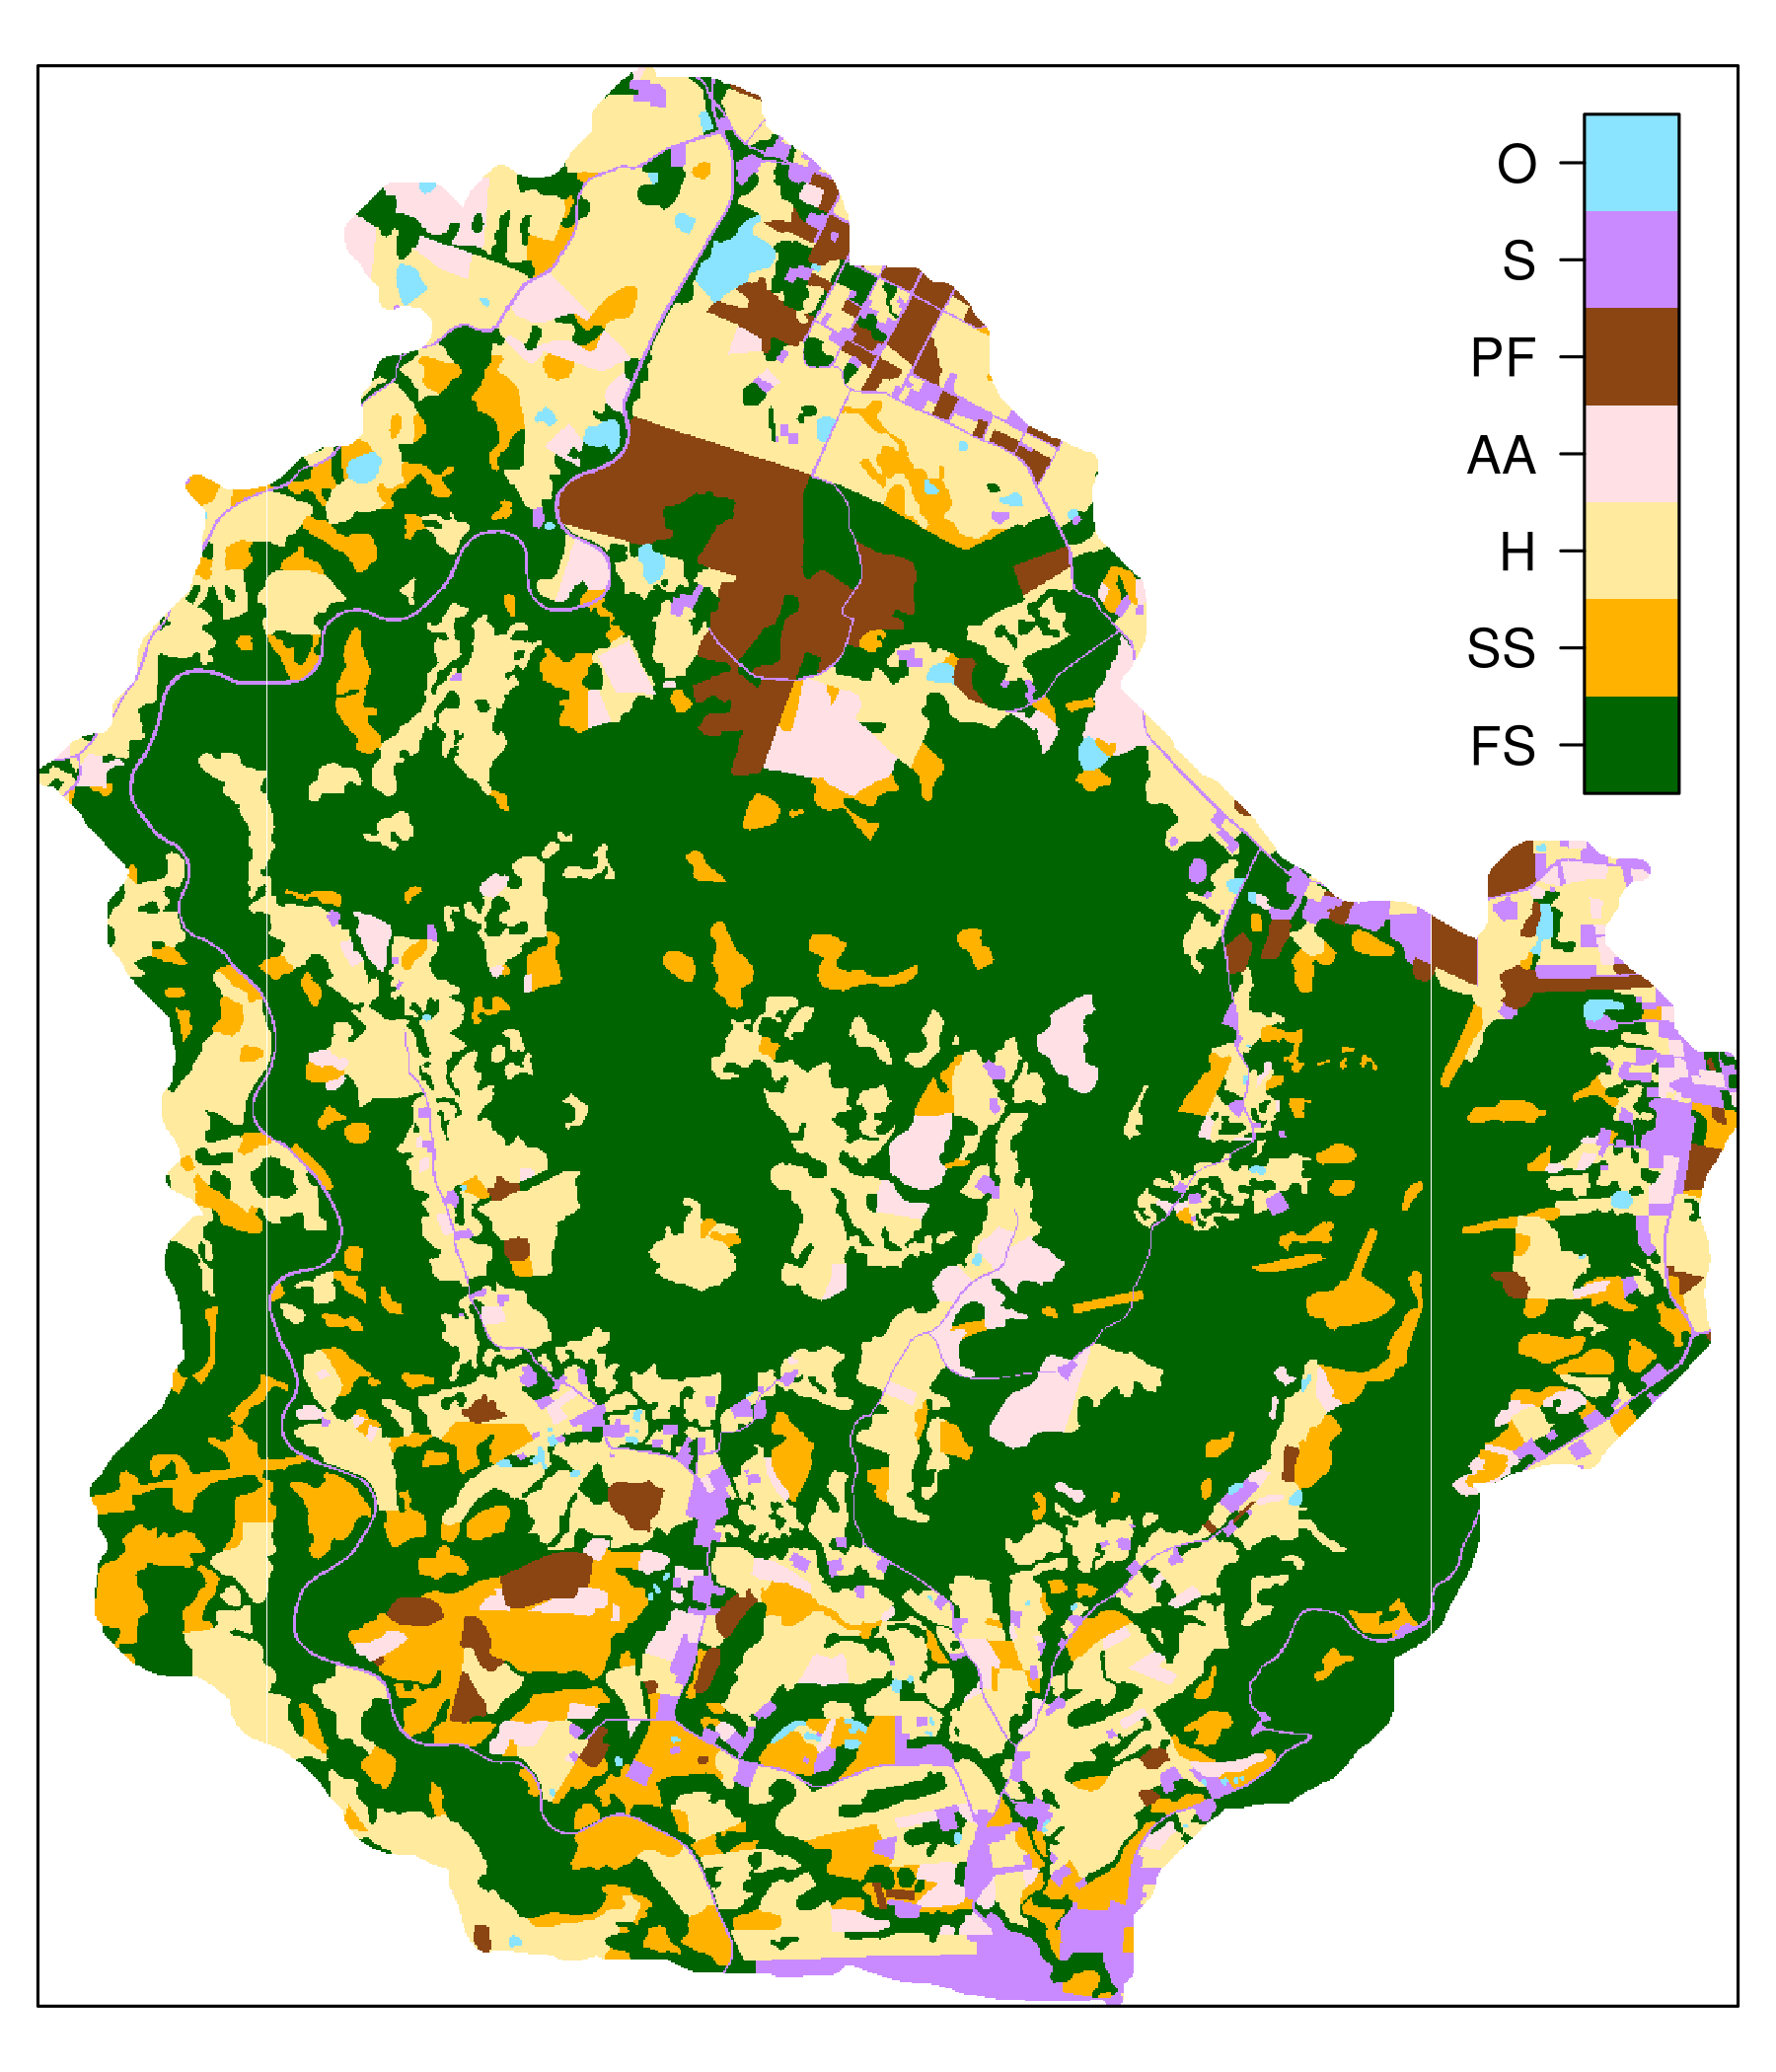
\includegraphics[width = \textwidth]{fig/chap05-land-new}
\end{minipage}
\begin{minipage}[b]{0.45\textwidth}
\subcaption{}
\label{fig:chap05-land-use-diff}
\centering
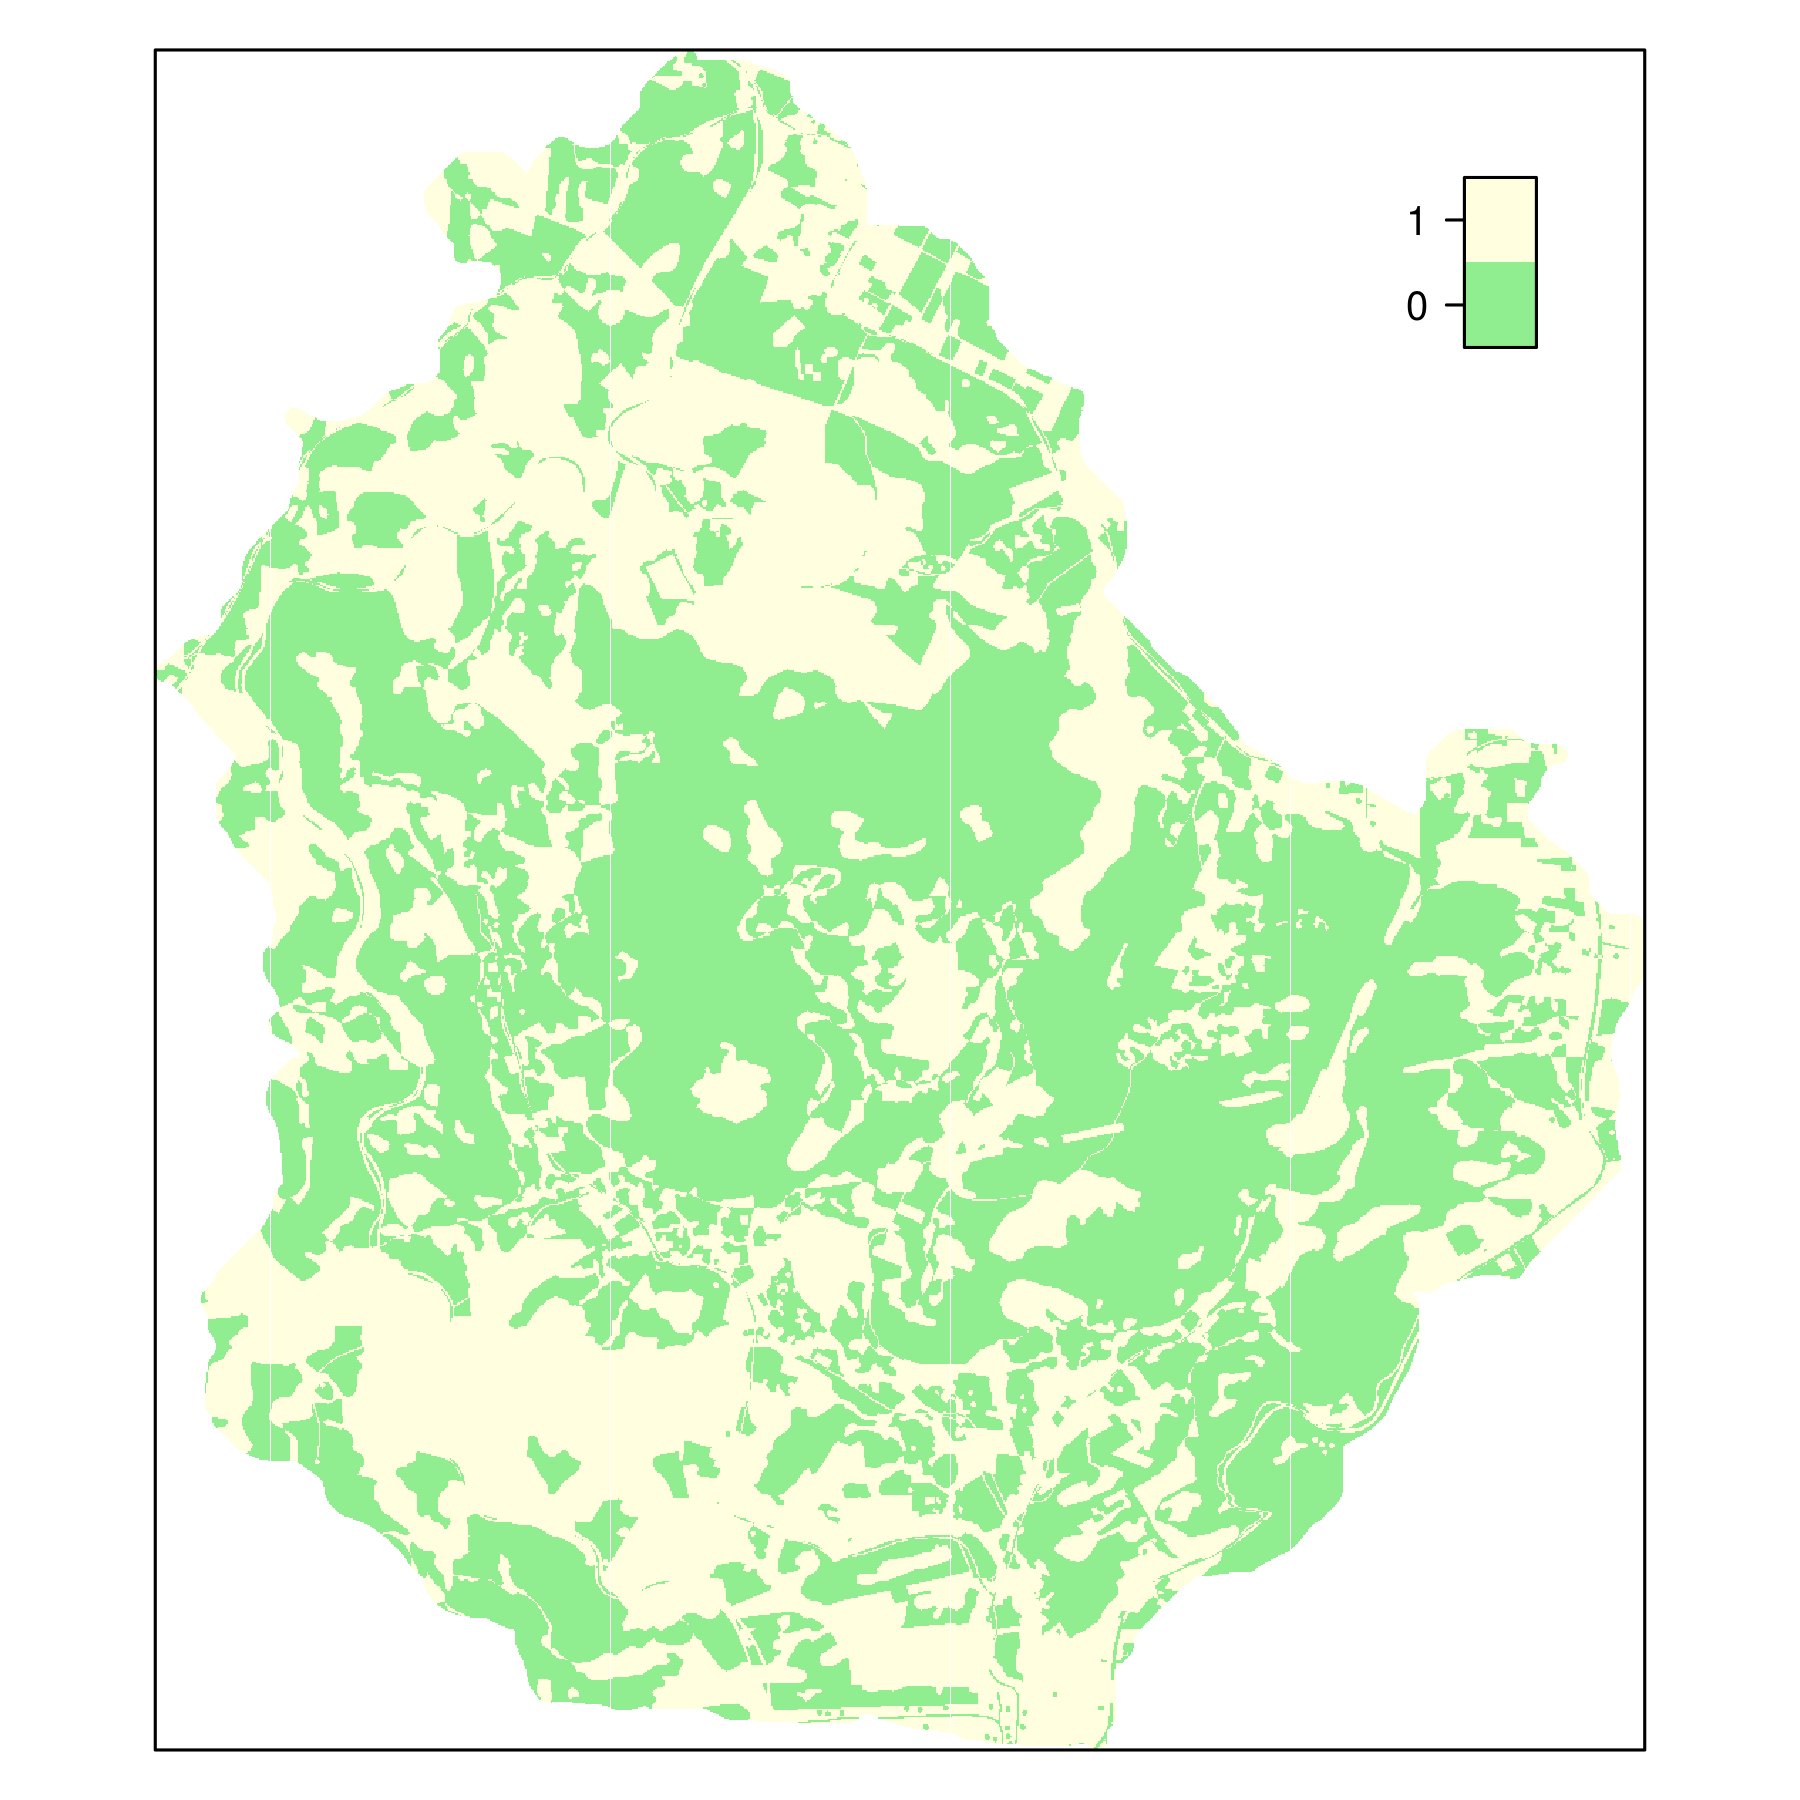
\includegraphics[width = \textwidth]{fig/chap05-land-diff}
\end{minipage}
\caption[Land use maps included in the Santa Maria dataset.]{Land use maps (a) \landOld{} and (b) \landNew{} 
used to derive indicator covariates included in the Santa Maria dataset such as (c) \texttt{LUdiff}, the land 
use change between the years of 1980 and 2009. Legend abbreviations and derived indicator variables are 
described in the text.}
\label{fig:chap05-land-use}
\end{figure}

The second land use map (\landNew{}, \autoref{fig:chap05-land-use-new}) was prepared at a \scale{2000} using 
high resolution (\SI{2.4}{\m}) Digital Globe\rr{} QuickBird satellite images of \num{2008} and \num{2009}, 
made publicly available in Google Earth\rr{} \cite{SamuelRosaEtAl2011a}. Identification of land uses and 
delineation of mapping units were done manually, on the computer screen, without using any automated 
classification routine. Positional validation of Google Earth\rr{} imagery revealed that they have only minor 
systematic positional errors (\autoref{tab:chap05-google-geo-val}). Despite of this, the attribute validation 
of both land use maps, using $n = 60$ validation points placed along $m = 12$ linear transects, showed that 
they have similar overall accuracy close to \SI{70.00}{\percent}.

\ctable[
  caption  = {Error statistics of the horizontal validation of Google Earth\rr{} imagery using $n = 14$ ground 
  control points.},
  cap      = {Error statistics of the horizontal validation of Google Earth\rr{} imagery.},
  label    = tab:chap05-google-geo-val,
  notespar,
  pos      = !ht,
  maxwidth = \textwidth,
  % doinside = \scriptsize\setstretch{1.1},
  doinside = \small
  ]{lrrrr}{
  }{                                                                          \FL
  Statistics                   & x-coord & y-coord & Error vector & Azimuth   \ML
  Mean, \si{\m}                & -1      & 3       & 6            & \ang{184} \NN
  Absolute mean, \si{\m}       & 3       & 5       & -            & -         \NN
  Squared mean, \si{\m\square} & 14      & 57      & 71           & -         \LL
  }

\landOld{} was used to derive $p = 2$ covariates defined as indicator variables, with plantation forests 
(\textit{PF}) and human settlements (\textit{S}) being grouped together due to their small importance in terms 
of covered area (\textit{PF}) and for not containing any soil observation (\textit{S}). These covariates are:

\begin{description}
\item[\texttt{LU1980a}] Native forest (\textit{FS}), which is likely to have soils with higher fertility.
  
\item[\texttt{LU1980b}] Animal husbandry (\textit{H}), the second most important land use in the study area, 
which is likely to have a soil fertility status lower than native forests.
\end{description}

Four ($p = 4$) indicator covariates were derived from \landNew{}, with plantation forests (\textit{PF}), human 
settlements (\textit{S}), and other land uses (\textit{O}), which comprise natural and artificial water 
bodies, being grouped together due to their small importance in terms of covered area (\textit{PF}) and for 
not containing any soil observation (\textit{S} and \textit{O}). These covariates are:

\begin{description}
\item[\texttt{LU2009a}] Native forest (\textit{FS}), as described above.
 
\item[\texttt{LU2009b}] Shrubland (\textit{SS}), which is likely to have a soil fertility level above those 
found in areas used with annual crop agriculture and animal husbandry, but lower than in native forests.
 
\item[\texttt{LU2009c}] Animal husbandry (\textit{H}), as described above.
  
\item[\texttt{LU2009d}] Annual crop agriculture (\textit{AA}), which is likely to present the lowest soil 
fertility levels due to the usually poor management practices employed.
\end{description}

A seventh indicator covariate (\texttt{LUdiff}, \autoref{fig:chap05-land-use-diff}) was derived using data 
from both land use maps. It consists of the land use change between \num{1980} and \num{2009}, computed by 
checking if the land use has changed (1) or remained the same (0) in every grid cell after the 29-year period. 
\texttt{LUdiff} can be useful, for example, to explain the low soil organic carbon content in forest soils due 
to previous use with crop agriculture or animal husbandry.

\section{SATELLITE IMAGES}
\label{sec:chap05-sat-image}

Two sources of satellite images were used to produce covariate data included in the Santa Maria dataset. The 
first is the Thematic Mapper (TM) sensor aboard the longest-operating Earth observation satellite -- Landsat 
5 (\autoref{fig:chap05-sat-old}). The satellite image used was acquired on \num{26} December \num{2010} and is 
freely available in the database of the Division of Image Generation of the Brazilian National Institute for 
Space Research (\inpedgi). The image contains seven spectral bands (\autoref{tab:chap05-satellites}) 
(including a thermal band that is not included in the Santa Maria dataset), with \SI{8}{\bit} radiometric 
resolution (digital numbers from \numrange{0}{255}) and \SI{30}{\m} spatial resolution. The satellite image 
was orthorectified using Geomatica\rr{} OrthoEngine\rr{} with the Landsat rigorous model (Toutin's Model) 
\cite{Toutin2004, PCIGeomatics2007}. Due to the absence of good identifiable field GCPs, $n = 28$ GCPs were 
collected from Google Earth\rr{} imagery, which have a high positional accuracy in the DNOS catchment 
(\autoref{tab:chap05-google-geo-val}). GCPs were located at easily identifiable geographical markers such as 
road intersections and bridges, evenly distributed throughout the image, and covering a variety of elevations, 
following standard recommendations \cite{PCIGeomatics2007}. 
% TODO: add link to \autoref{fig:chap05-ortho-gcps}
The DEM used for orthorectification is TOPODATA after preprocessing as described in \autoref{sec:chap05-dem}. 
Resampling was done using the nearest neighbour method to avoid changing the digital numbers.

After orthorectification, all bands were imported into GRASS GIS, where all other necessary corrections were 
performed. Radiometric correction (conversion from digital numbers to top-of-atmosphere reflectance) was done 
using \grass{i.landsat.toar}. Atmospheric correction (removal of the effects of the atmosphere on the 
reflectance values) was done with the 6S atmospheric model \cite{VermoteEtAl1997} as implemented in 
\grass{i.atcorr} using the tropical atmospheric model, the continental aerosols model, an image-based 
visibility estimate of \SI{20}{\km}, and a constant elevation of \SI{300}{\m}.

The second source of satellite images is RapidEye (\autoref{fig:chap05-sat-new}). Images are available through 
the Brazilian Ministry of the Environment \cite{Brasil2012}, which has a full coverage of the Brazilian 
territory for \num{2011} and \num{2012}. The satellite image used (tile number \num{2225403}) was acquired on 
\num{16} November \num{2012} (second coverage). It contains five spectral bands 
(\autoref{tab:chap05-satellites}), featuring among them the so-called red-edge band, located between the red 
and the near-infrared bands. This spectral band is the main feature distinguishing RapidEye images from most 
other sources of satellite images, considered to provide additional information about the vegetation 
\cite{WeicheltEtAl2013}. The satellite image has \SI{16}{\bit} radiometric resolution and \SI{6.5}{\m} spatial 
resolution, and was orthorectified at the source to \SI{5}{\m} spatial resolution using the sink-filled SRTM 
version \num{4} DEM \cite{RapidEye2013}.

\begin{figure}[!ht]
\centering
\begin{minipage}[b]{0.45\textwidth}
\subcaption{}
\label{fig:chap05-sat-old}
\centering
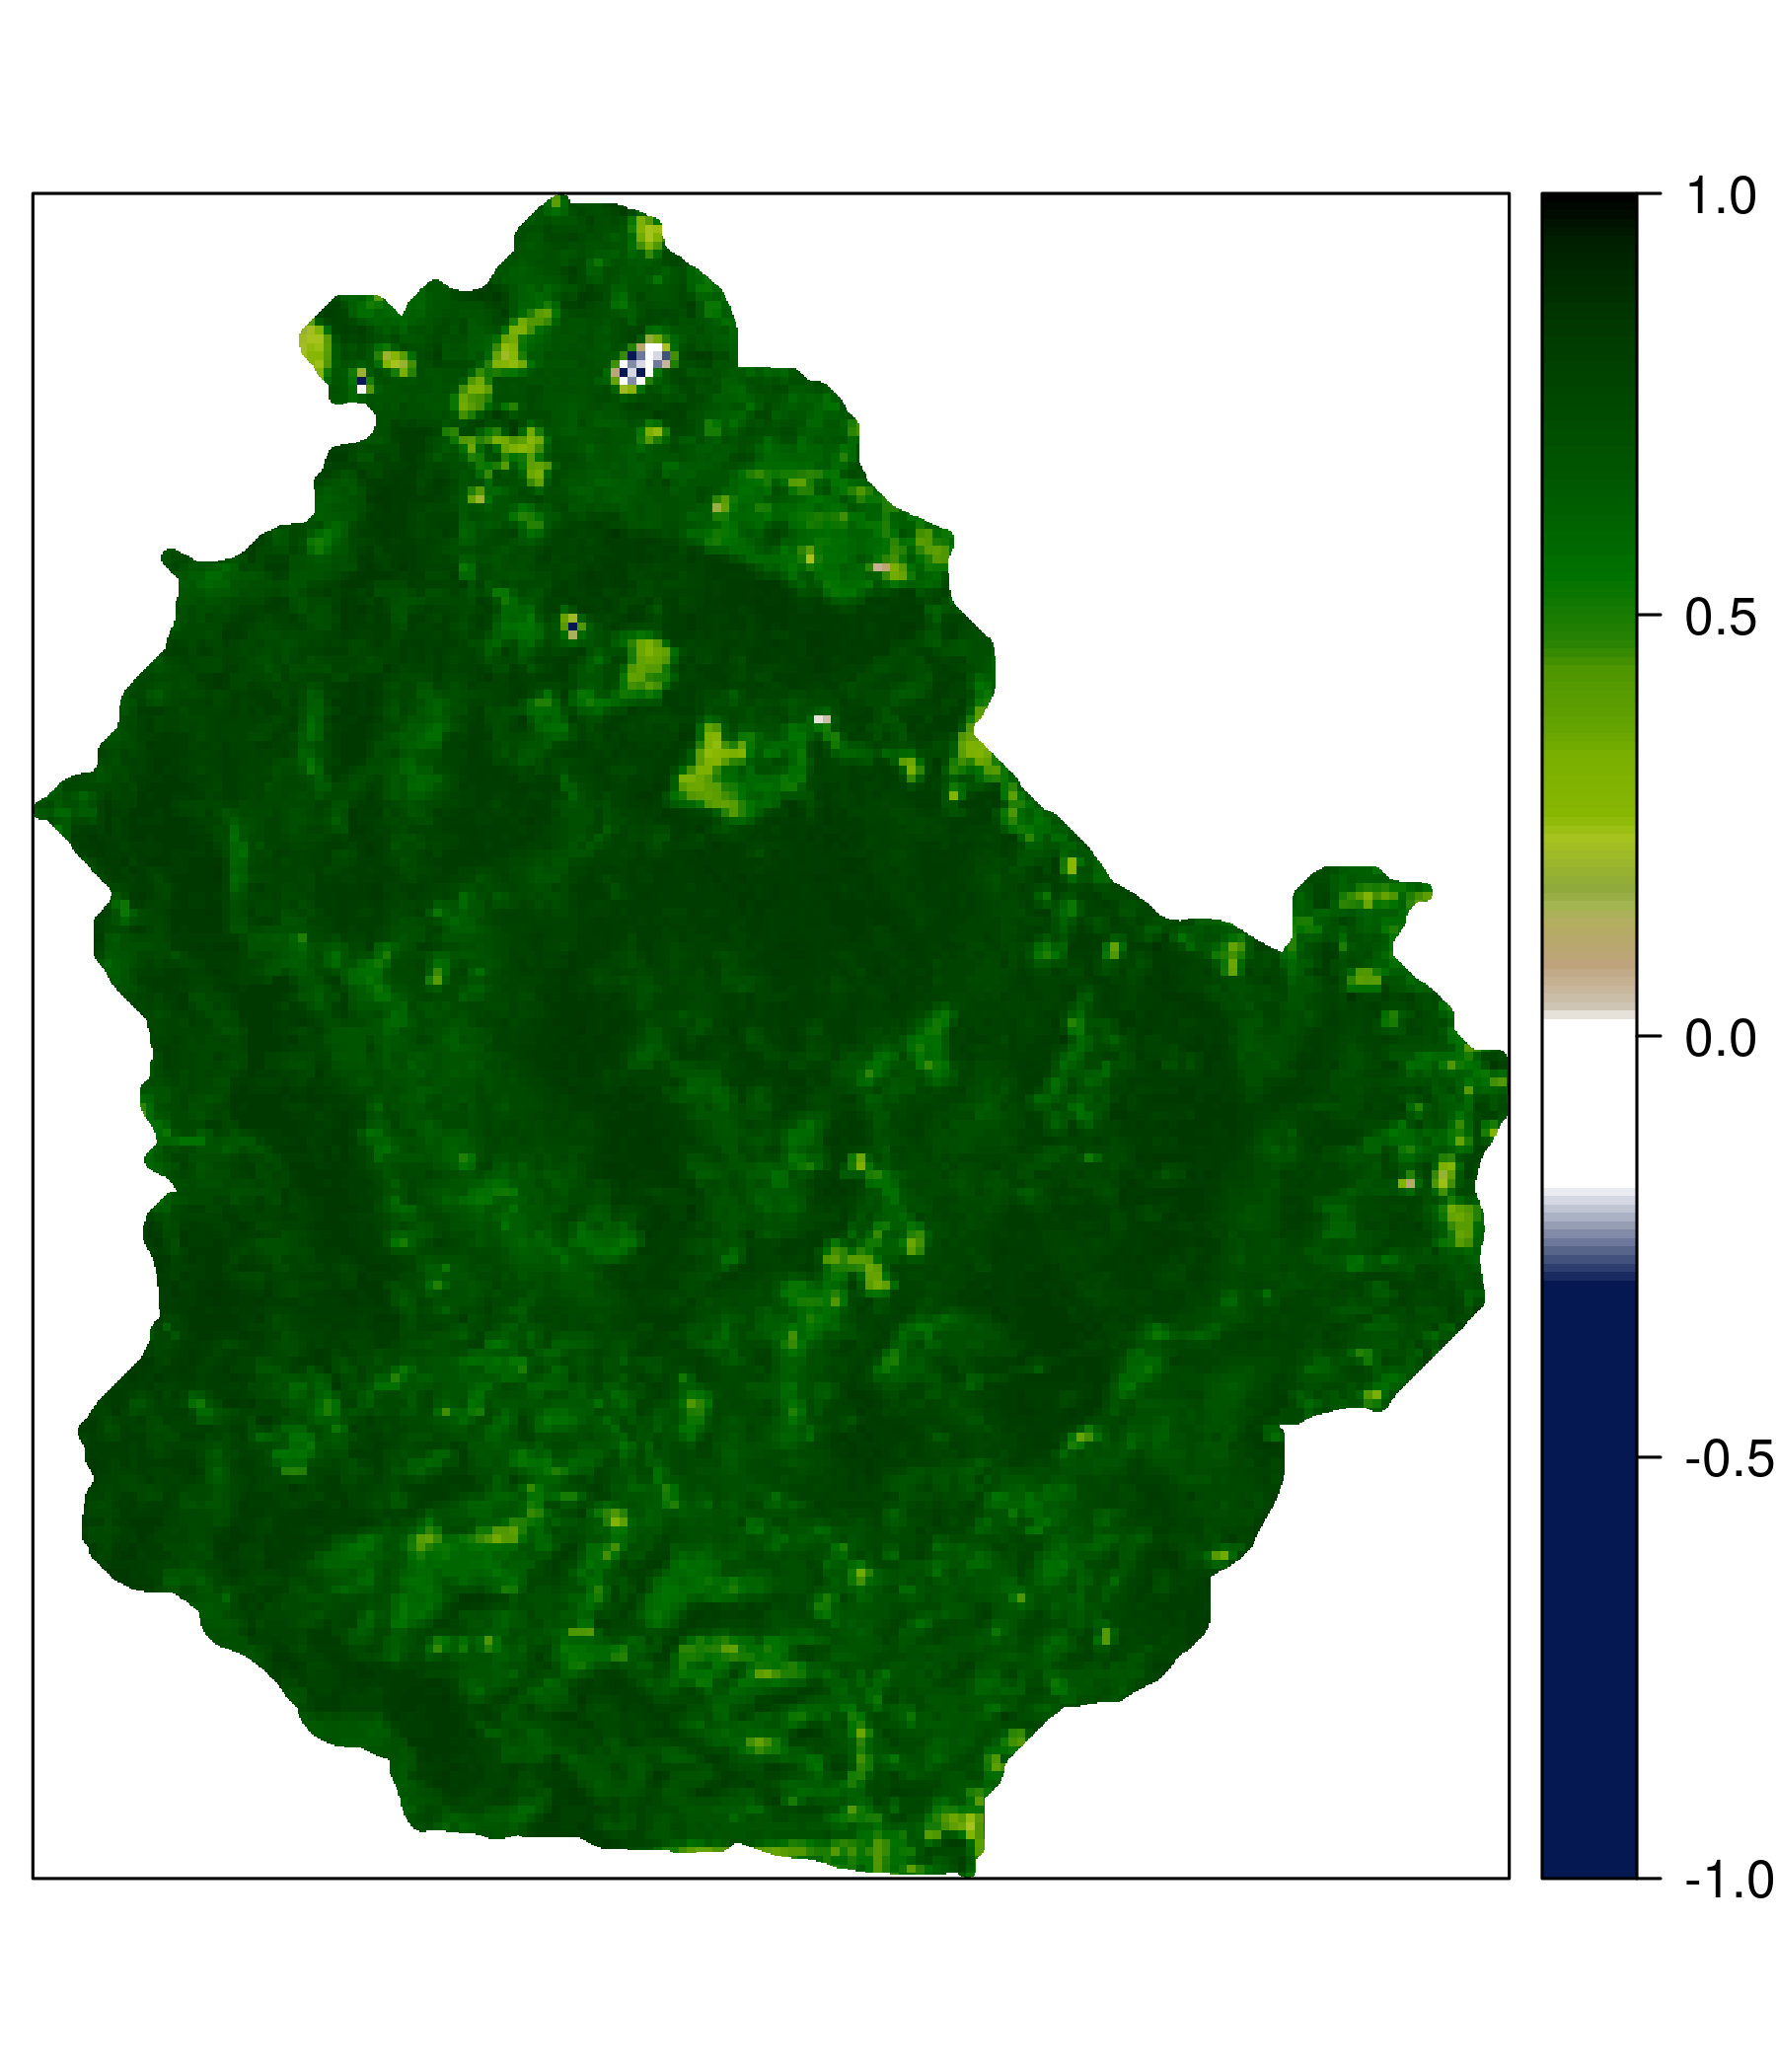
\includegraphics[width = \textwidth]{fig/chap05-sat-old}
\end{minipage}
\begin{minipage}[b]{0.45\textwidth}
\subcaption{}
\label{fig:chap05-sat-new}
\centering
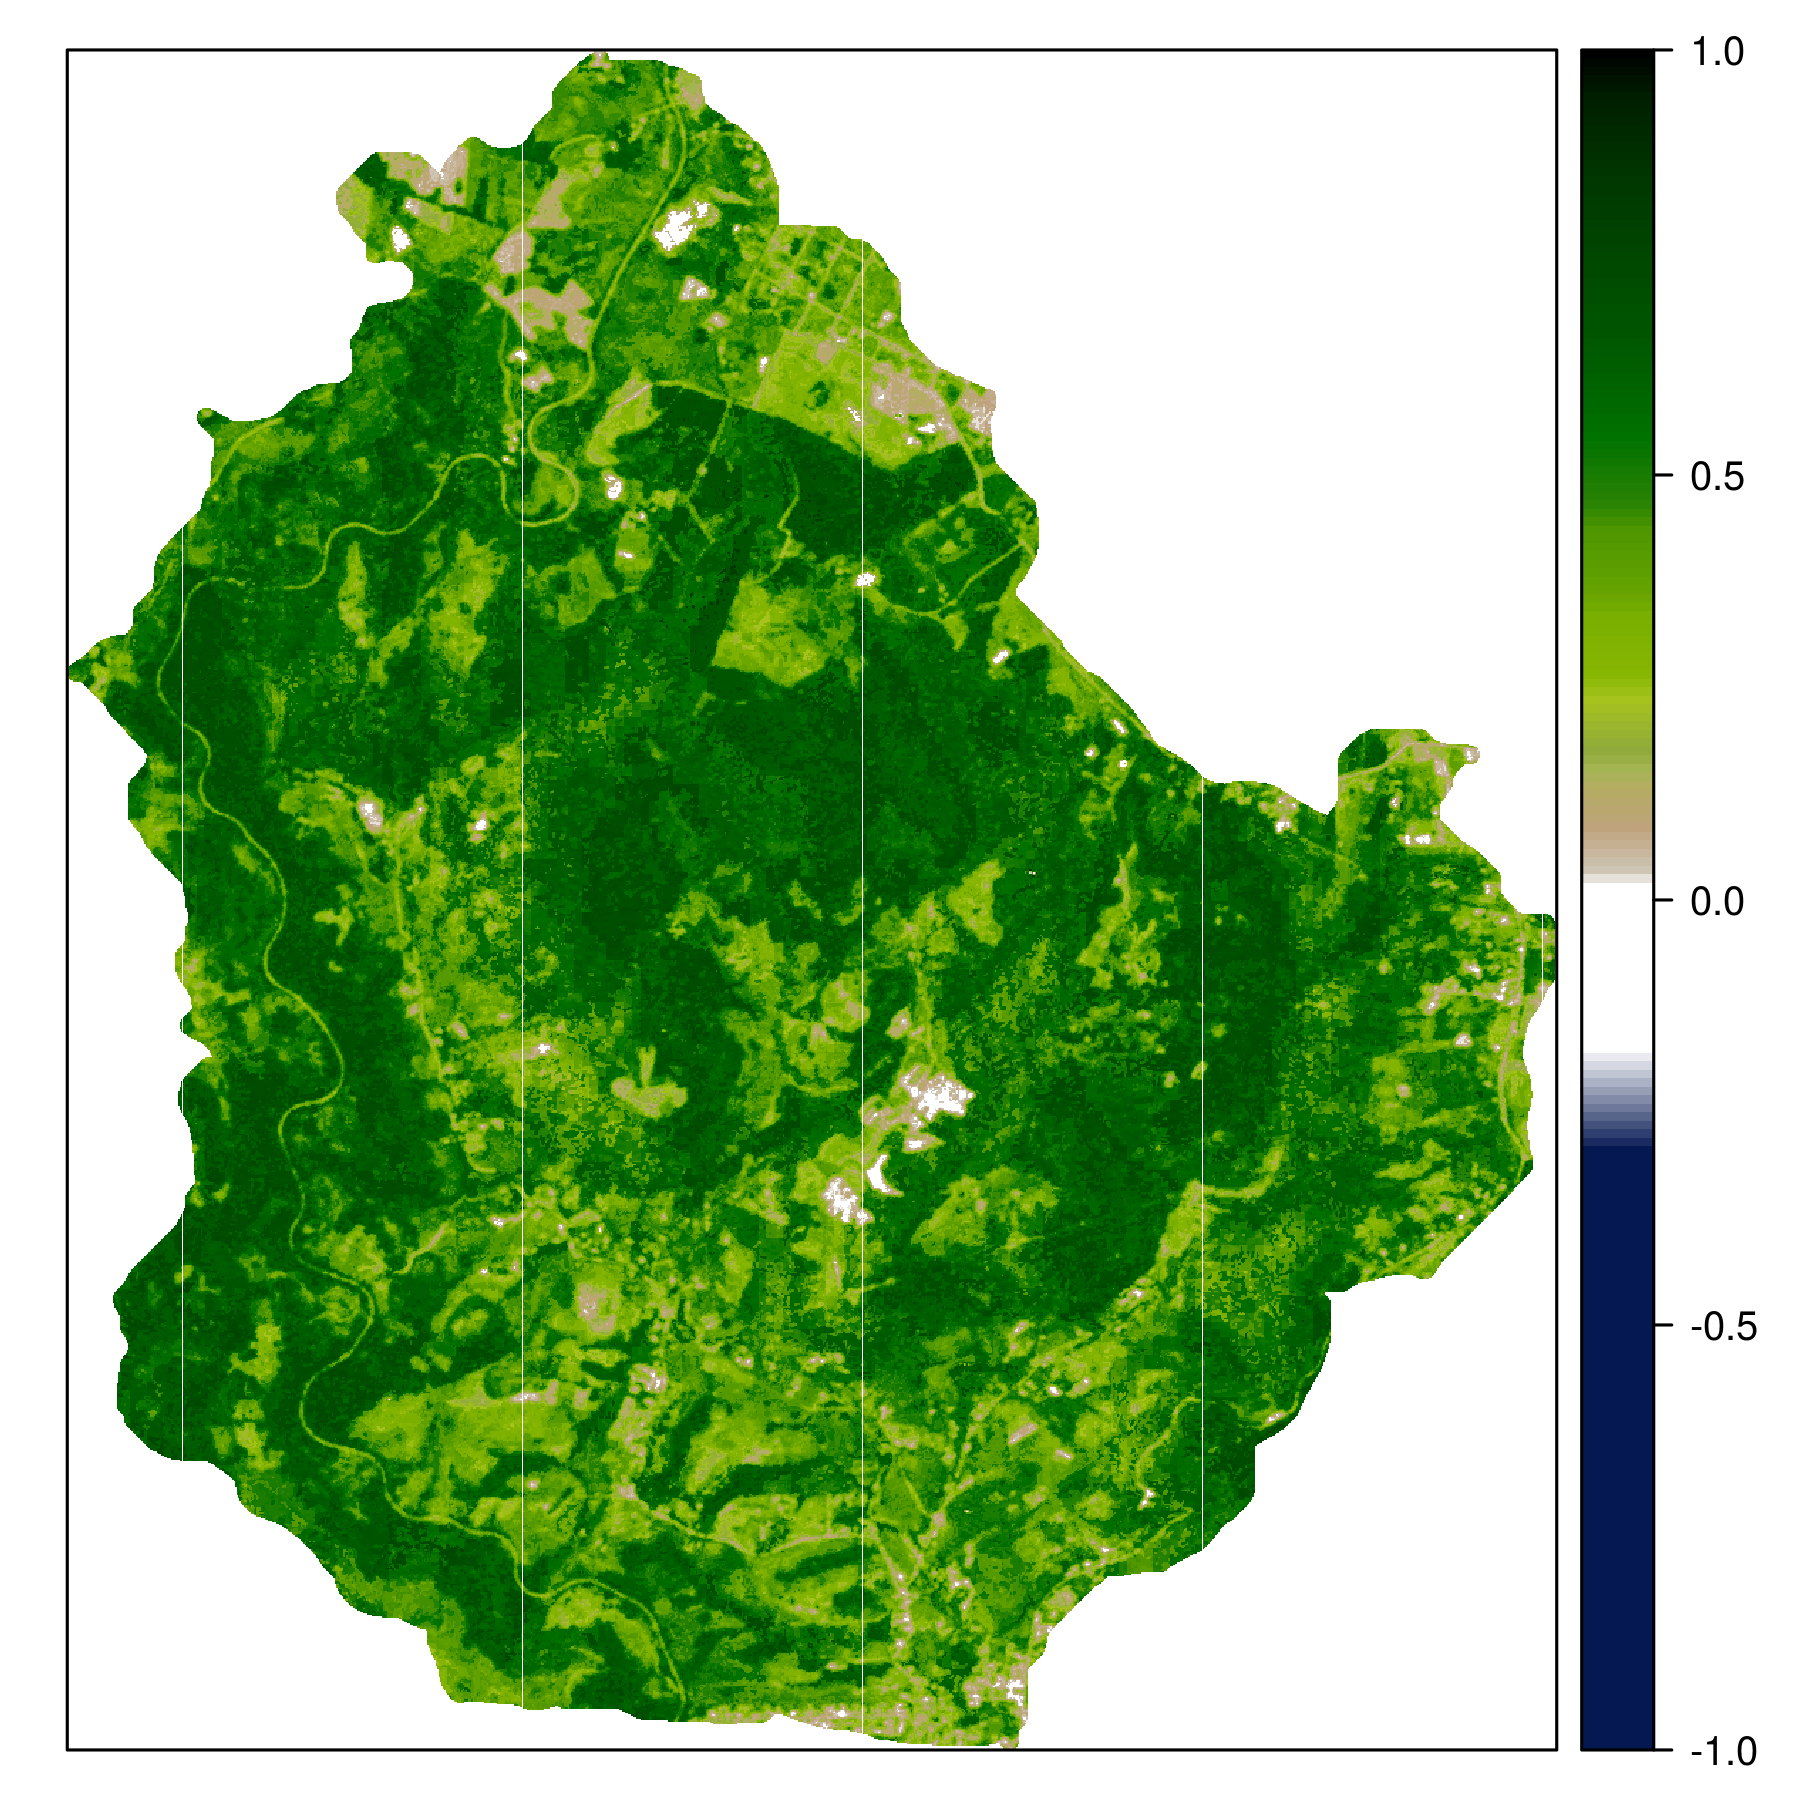
\includegraphics[width = \textwidth]{fig/chap05-sat-new}
\end{minipage} 
\caption[Satellite images included in the Santa Maria dataset.]{Satellite images used to derive covariates 
such as (a) \texttt{NDVI\_30} and (b) \texttt{NDVI\_5b} included in the Santa Maria dataset.}
\label{fig:chap05-sat-image}
\end{figure}

\ctable[
  caption  = {Comparison between satellite images produced by Landsat 5 TM and RapidEye and the derived 
  covariates.},
  cap      = {Comparison between satellite images and derived covariates.},
  label    = tab:chap05-satellites,
  notespar,
  pos      = !ht,
  maxwidth = \textwidth,
  % doinside = \scriptsize\setstretch{1.1},
  doinside = \small
  ]{lllllll}{
  }{ \FL
  \multicolumn{3}{l}{Landsat 5 TM}                  && \multicolumn{3}{l}{RapidEye} \NN
  \cmidrule(r){1-3}\cmidrule(l){5-7}
  Band & Interval, \si{nm} & Covariate              && Band & Interval, \si{\nm} & Covariate \ML
  1 Visible       & 450--520   & \texttt{BLUE\_30}  && Blue & 440--510 &\texttt{BLUE\_5} \NN
  2 Visible       & 520--600   & \texttt{GREEN\_30} && Green & 520--590& \texttt{GREEN\_5} \NN
  3 Visible       & 630--690   & \texttt{RED\_30}   && Red & 630--685 & \texttt{RED\_5} \NN
  -               & -          & -                  && Red-edge & 690--730 & \texttt{EDGE\_5} \NN
  4 Near-infrared & 760--900   & \texttt{NIR\_30a}  && Near-infrared & 760--850 & \texttt{NIR\_5} \NN
  5 Near-infrared & 1550--1750 & \texttt{NIR\_30b}  && - & - & - \NN
  7 Mid-infrared  & 2080--2350 & \texttt{MIR\_30}   && - & - & - \LL
  }

The RapidEye image was atmospherically corrected using the 6S atmospheric model \cite{VermoteEtAl1997} 
employing the Fortran code developed by \citeonline{AntunesEtAl2013} -- \grass{i.atcorr} was not used because 
a \atcorrbug{} was found when trying to correct the RapidEye image -- assuming a tropical atmospheric model, 
the continental aerosols model, an image-based visibility estimate of \SI{20}{\km}, and a constant elevation 
of \SI{300}{\m}.

After atmospheric correction, Landsat 5 TM and RapidEye images were resampled using the nearest neighbour 
method to match the reference grid. Topographic correction was performed using \grass{i.topo.corr} with 
TOPODATA geometrically corrected to match the reference grid as described in \autoref{sec:chap05-dem}.

\ctable[
  caption  = {Error statistics of the horizontal validation of satellite images produced by Landsat 5 TM and 
  RapidEye using $n = 14$ ground control points.},
  cap      = {Error statistics of the horizontal validation of satellite images.},
  label    = tab:chap05-satellite-geo-val,
  notespar,
  pos      = !ht,
  maxwidth = \textwidth,
  % doinside = \scriptsize\setstretch{1.1},
  doinside = \small
  ]{lrrrr}{
  }{ \FL
  Statistics                   & x-coord & y-coord  & Error vector  & Azimuth   \ML
  \multicolumn{5}{l}{Landsat 5 TM}                                              \ML
  Mean, \si{\m}                & 31      & -11      & 45            & \ang{136} \NN
  Absolute mean, \si{\m}       & 33      & 25       & -             & -         \NN
  Squared mean, \si{\m\square} & 1494    & 1223     & 2717          & -         \ML
  \multicolumn{5}{l}{RapidEye}                                                  \ML
  Mean, \si{\m}                & -25     & -25      & 36            & \ang{226} \NN
  Absolute mean, \si{\m}       & 25      & 25       & -             & -         \NN
  Squared mean, \si{\m\square} & 680     & 708      & 1388          & -         \LL
  } 

Individual bands of both satellite images were defined as covariates, totalling $p = 6$ from Landsat 5 TM and 
$p = 5$ from RapidEye (Table \ref{tab:chap05-satellites}). Another $p = 6$ covariates ($p = 2$ from Landsat 5 
TM and $p = 4$ from RapidEye) were defined using two vegetation indices: the normalized difference vegetation 
index (NDVI) and the soil-adjusted vegetation index (SAVI), calculated as

\begin{equation}\label{eqn:ndvi}
 \text{NDVI} = \frac{\text{NIR} - \text{RED}}{\text{NIR} + \text{RED}}
\end{equation}

\noindent and 

\begin{equation}\label{eqn:savi}
  \text{SAVI} = (1.0 + 0.5) \times \frac{\text{NIR} - \text{RED}}{\text{NIR} + \text{RED} + 0.5},
\end{equation}

\noindent where $\text{NIR} = \texttt{NIR\_30a}$ and $\text{RED} = \texttt{RED\_30}$ for the Landsat 5 TM 
image, and $\text{NIR} = \texttt{NIR\_5}$ and $\text{RED} = \texttt{RED\_5}$ or $\text{RED} = 
\texttt{EDGE\_5}$ for RapidEye image.

% \section{CONCLUSIONS}

% This document presented a thorough description of the covariate data (area-class soil maps, digital 
% elevation models, geological maps, land use maps, and satellite images) contained in the Santa Maria 
% dataset. This description included the procedures employed in their production, as well as all processing 
% methods employed. We expect the reader to have understood the features of the covariate data used in the 
% thesis, and that this description will support future soil spatial modelling exercises in the catchment of 
% the DNOS reservoir.

% As a result of an ongoing collaborative effort, it is likely that, as new studies are developed, this 
% documentation will be improved. For example, we already plan to include more figures with the indicator 
% covariates derived from area-class soil maps, geological maps and land use maps. Other DEM derivatives might 
% be included as well to better exemplify the effect of the window size on the spatial variation of calculated 
% DEM derivatives. Finally, we plan to include descriptive statistics of soil properties as related to the 
% different covariates as a means of improving our understanding of their empirical relationship.
